%=================================================================
\documentclass[remotesensing,article,submit,pdftex,moreauthors]{Definitions/mdpi} 
\usepackage{textcomp}
\usepackage{caption}
\usepackage{subcaption}
\usepackage{graphicx}
\usepackage{siunitx}
\usepackage{tabularx}
\usepackage{makecell}

\sisetup{table-number-alignment=center}


%\documentclass[preprints,article,submit,pdftex,moreauthors]{Definitions/mdpi} 

%--------------------
% Class Options:
%--------------------

\firstpage{1} 
\makeatletter 
\setcounter{page}{\@firstpage} 
\makeatother
\pubvolume{1}
\issuenum{1}
\articlenumber{0}
\pubyear{2025}
\copyrightyear{2025}
\datereceived{ } 
\daterevised{ } 
\dateaccepted{ } 
\datepublished{ } 
\hreflink{https://doi.org/} 

%=================================================================
% Full title of the paper (Capitalized)
\Title{Physically-Constrained Calibration and Transferability of a Semi-Analytical TSS Retrieval Model in a Tropical Coastal Lagoon System: Ciénaga Grande de Santa Marta, Colombia}

\TitleCitation{Title}

% Authors
\Author{
Jhonnatan Rodríguez$^{1}$, 
Luis J. Otero$^{2}$, 
Ana Carolina Torregroza-Espinosa$^{3}$, 
Juan C. Restrepo$^{2}$, 
Antonello Bruschi$^{4,*}$
}

\AuthorNames{
Jhonnatan Rodríguez, 
Luis J. Otero, 
Ana Carolina Torregroza-Espinosa, 
Juan C. Restrepo, 
Antonello Bruschi
}

\AuthorCitation{
Rodríguez, J.; 
Otero, L. J.; 
Torregroza-Espinosa, A. C.; 
Restrepo, J. C.; 
Bruschi, A.
}

\address{
$^{1}$ Department of Civil, Constructional and Environmental Engineering, 
Sapienza University of Rome, Rome, Italy; 
\texttt{jhonnatan.rodriguezramos@uniroma1.it}\\

$^{2}$ Departamento de Física y Geociencias, Universidad del Norte, 
Barranquilla, Colombia\\

$^{3}$ Departamento de Ciencias Naturales y Exactas, 
Corporación Universidad de la Costa (CUC), 
Barranquilla 080001, Colombia\\

$^{4}$ Istituto Superiore per la Protezione e la Ricerca Ambientale (ISPRA), 
Via Vitaliano Brancati 48 and 60, 00144 Rome, Italy
}

\corres{
Correspondence: 
jhonnatan.rodriguezramos@uniroma1.it
}

% Keywords
\abstract{Empirical TSS retrieval models derived from satellite reflectance are frequently applied beyond their calibration domain without explicit assessment of parameter identifiability or rigorous transferability testing. We address both limitations using harmonised Landsat-8 (L8) and Sentinel-2 (S2) matchup datasets collected at the Pajarales sub-lagoon (calibration; n = 240) and the Ciénaga Grande de Santa Marta (CGSM; validation; n = 74, 2015–2024), Colombia. We introduce a formal identifiability criterion ($\kappa = \rho_{max}/C_{p,upper} \geq  0.35$) to determine whether the Nechad saturation parameter $C_p$ can be reliably estimated from data; when $\kappa < 0.35$, a closed-form weighted least-squares solution for the amplitude parameter $A_p$ alone is applied, with $C_p$ fixed to the band's physical upper bound rather than the literature value, which was found to destabilise the fit for this system. Landsat-8 and Sentinel-2 are calibrated and reported as separate, physically grounded single-sensor models rather than pooled into a single retrieval, since a pooled fit was found to underperform either sensor calibrated alone. A systematic four-scenario transferability framework — spanning direct parameter transfer, local recalibration, partial transfer, and a machine-learning benchmark — reveals a monotonic gradient in leave-one-station-out performance at the CGSM: direct transfer with no local adjustment achieves $R^2 = 0.448$; partial transfer (fixed $C_p$ from Pajarales, locally refitted $A_p$) reaches $R^2 = 0.531$; full local recalibration reaches $R^2 = 0.639$, closely approaching the Landsat-8 calibration ceiling at Pajarales itself ($R^2 = 0.662$); and a Gradient Boosting ceiling reaches $R^2 = 0.681$. This smooth degradation, rather than a catastrophic failure of direct transfer, follows from anchoring $C_p$ at a value that remains numerically stable across both sites. Analysis of 10 years of in-situ matchups (2015–2024) reveals significantly higher dry-season TSS (median 75 mg/L) than wet-season values (29 mg/L; Kruskal-Wallis p < 0.001) in Pajarales, while the CGSM shows weaker seasonal differentiation. An atmospheric-correction artefact was identified and corrected for Sentinel-2 at Pajarales, after which Sentinel-2 reflectance--TSS correlation improved from r = 0.12 to r = 0.62; even so, Landsat-8 retains substantially stronger and more stable performance ($R^2_{\text{LOSO}} = 0.662$ vs.\ $0.372$), and a persistent inter-sensor reflectance offset precludes pooled multi-sensor calibration at this site. These findings provide a reproducible, physics-grounded calibration and transfer framework applicable to data-limited tropical coastal lagoons.}
\keyword{Remote sensing, Water quality, Environmental monitoring, Time Series Analysis, Seasonal Dynamics, Landsat 8, Sentinel 2} 

%%%%%%%%%%%%%%%%%%%%%%%%%%%%%%%%%%%%%%%%%%
\begin{document}
\section{Introduction}

Coastal lagoon systems are among the most spatially and temporally
dynamic aquatic environments, exhibiting rapid fluctuations in water
quality driven by hydrodynamic exchange, riverine inputs, and
meteorological forcing \citep{Barbier2011, Barbier2017}.
Total Suspended Solids (TSS) constitute a key optically active
constituent in these systems, governing light penetration, primary
productivity, and biogeochemical cycling \citep{Arias2022}.
Satellite-based TSS retrieval has become an established tool for
synoptic monitoring, with operational approaches ranging from empirical
regression to semi-analytical bio-optical models \citep{Pahlevan2022, adjovu}.
However, two fundamental methodological challenges limit the reliability
of empirical TSS models in data-limited environments: parameter
identifiability and spatial transferability \citep{Arias2022, Hua2017}.
 
These challenges are amplified in tropical coastal lagoons, where
sediment dynamics are strongly modulated by hydrological and climatic
variability. River discharge, precipitation anomalies, wind-driven
resuspension, and extreme meteorological events can substantially alter
sediment loads and turbidity patterns \citep{Yunus2021, Li2021}. In
shallow systems, where bottom resuspension and rapid hydrodynamic
fluctuations are common, TSS concentrations may vary considerably over
short temporal scales, introducing substantial uncertainty in water
quality assessments and predictive modelling.
 
Traditional water quality monitoring based on \textit{in situ} sampling
provides accurate point-based measurements; however, it remains
spatially sparse and temporally discontinuous, limiting its ability to
capture the high spatiotemporal variability characteristic of tropical
lagoon systems \citep{Arias2022}. Satellite remote sensing has therefore
emerged as a powerful complementary tool for long-term synoptic
monitoring of optically active water constituents. Numerous studies have
demonstrated empirical relationships between TSS and visible--near
infrared (VNIR) reflectance derived from Landsat and Sentinel-2 imagery
\citep{adjovu,Li2021}.
Nevertheless, retrieving TSS from satellite observations in optically
complex coastal waters remains challenging due to variations in particle
composition, bottom reflectance in shallow areas, coloured dissolved
organic matter (CDOM), atmospheric correction uncertainties, and
sensor-specific spectral responses.
 
Recent advances in atmospheric correction algorithms, particularly
ACOLITE \citep{Vanhellemont2015, Vanhellemont2019}, have improved the
retrieval of water-leaving reflectance in turbid coastal and estuarine
waters, enabling more reliable estimation of suspended sediments from
medium-resolution satellite imagery. However, empirical TSS retrieval
models are frequently site-specific, raising concerns regarding their
transferability across spatially heterogeneous environments.
Additionally, the integration of multi-sensor datasets introduces
further complexity due to differences in spectral configuration,
radiometric consistency, and atmospheric correction sensitivity between
Landsat-8 and Sentinel-2.
 
Although several studies have explored TSS dynamics and sensor
harmonisation approaches, important methodological limitations remain
unresolved. Most studies rely on strict same-day satellite--\textit{in
situ} matchups, which substantially reduce sample size and limit model
robustness, particularly in tropical regions persistently affected by
cloud cover \citep{Pahlevan2022}. Furthermore, the spatial
transferability of empirical models is rarely evaluated using
independent cross-validation, despite representing a critical
requirement for operational monitoring. A further limitation that has
received insufficient attention is the identifiability of semi-analytical
model parameters: when observed reflectances span only the near-linear
segment of the calibration function, individual parameters cannot be
reliably estimated from data, leading to physically meaningless fitted
values that may nonetheless appear numerically plausible.
 
Suspended sediment dynamics in the CGSM are also influenced by
large-scale hydroclimatic variability, including seasonal wind patterns
and interannual anomalies associated with the El~Ni\~{n}o--Southern
Oscillation (ENSO), which modulate freshwater inputs and resuspension
processes \citep{Blanco2006}. Characterising these seasonal patterns
from satellite-matched field observations contributes to a more complete
understanding of long-term sediment dynamics in the system.
 
The CGSM, a Ramsar-listed coastal lagoon complex of global ecological
importance, exemplifies these challenges. Despite extensive research
addressing its hydrology, ecology, geomorphology, and biogeochemistry
\citep{Gonima1998, Blanco2006, Jaramillo2018, Espinoza2025}, no previous
study has (i)~explicitly assessed the identifiability of Nechad model
parameters for this system, (ii)~evaluated model transferability between
sub-lagoon sectors under a systematic multi-scenario cross-validated
framework, or (iii)~characterised seasonal and interannual TSS
variability from harmonised multi-sensor matchup datasets spanning a
decade.
 
To address these gaps, this study introduces a temporally weighted
calibration framework incorporating satellite observations acquired
within a $\pm$2.5-day window relative to \textit{in situ} measurements.
This approach increases the number of valid satellite--field matchups
while explicitly accounting for the uncertainty introduced by
non-coincident observations through exponential temporal weighting.
Empirical TSS retrieval models were developed within the Pajarales
sub-lagoon and their transferability to the central CGSM was evaluated
under four explicitly defined scenarios.
 
A critical aspect of this work is the explicit consideration of
uncertainties arising from temporal mismatches between satellite and
\textit{in situ} observations, limited spatial representativeness of
validation datasets, and the constraints imposed by limited reflectance
dynamic range on model parameter estimation. By addressing these
constraints, this study contributes a reproducible and
physically-grounded framework for multi-sensor TSS monitoring in
data-limited tropical estuarine environments.
 
To the best of our knowledge, this represents the first study to
(i)~apply a formal identifiability criterion to Nechad parameter
estimation in this system, (ii)~evaluate TSS model transferability
between CGSM sub-lagoons using a systematic four-scenario
cross-validated framework, and (iii)~characterise the
sensor-specific performance gap between harmonised Landsat-8 and
Sentinel-2 matchup datasets in tropical turbid waters.
 
Accordingly, the objectives of this study are to:
 
\begin{itemize}
    \item Develop and cross-validate empirical TSS retrieval models
          using a temporally weighted satellite--\textit{in situ}
          calibration framework, with explicit identifiability
          assessment of Nechad model parameters.
 
    \item Evaluate the spatial transferability of the calibrated models
          from the Pajarales sub-lagoon to the central CGSM under four
          systematically defined scenarios, distinguishing between
          direct transfer, partial parameter transfer, local
          recalibration, and a machine-learning benchmark.
 
    \item Characterise seasonal and interannual TSS variability from
          ten years of satellite-matched \textit{in situ} observations
          (2015--2024) across both sub-lagoon systems.
 
    \item Assess the performance consistency between Landsat-8 and
          Sentinel-2 within the harmonised calibration framework and
          identify the conditions under which joint multi-sensor
          calibration is appropriate.
\end{itemize}
%%%%%%%%%%%%%%%%%%%%%%%%%%%%%%%%%%%%%%%%%%
\section{Materials and Methods}
\subsection{Study Area}

The Ci\'{e}naga Grande de Santa Marta (CGSM) is located at
$10^\circ52'00''\,\text{N},\ 74^\circ25'00''\,\text{W}$,
with a surface area of approximately 205{,}393~ha (INVEMAR, unpublished
data) and an average depth between 1.8 and 2.3~m. The lagoon's extent
fluctuates seasonally in response to variations in freshwater inflows
and evapotranspiration. Freshwater is primarily supplied by rivers such
as Fundaci\'{o}n, Sevilla, and Aracataca, while saline water intrusion
occurs from the Caribbean Sea. This interplay shapes the spatial and
temporal salinity gradients that underpin the lagoon's ecological
complexity and productivity \citep{Tuchkovenko2003}.
 
Dominated by extensive mangrove forests \citep{Gonima1998, Konnerup2014},
CGSM provides habitat for diverse fauna, including commercially valuable
species. The region's arid to semi-arid climate is
characterised by average temperatures of
26.8--34.9\,\textdegree C and high evapotranspiration rates, which
contribute to a persistent water deficit despite seasonal rainfall
\citep{Hernandez1990}.
 
Within the broader CGSM deltaic system lies the Pajarales Complex (CP),
located between $10^\circ45'\,\text{N}$--$11^\circ00'\,\text{N}$ and
$74^\circ30'\,\text{W}$--$74^\circ40'\,\text{W}$
\citep{Invemar2014},
covering approximately 15{,}279~ha. Bordered by the Isla de Salamanca
National Natural Park to the north and the CGSM Fauna and Flora
Sanctuary to the south, CP is hydrologically connected to the CGSM
through surface and subsurface channels, and also receives freshwater
inflows from the Magdalena River to the west.
 
The CP's geomorphology consists of shallow wetlands (1.8--5.0~m deep)
with muddy substrates and mangrove-fringed margins. Its hydroclimatic
regime mirrors that of CGSM, with a pronounced dry season
(January--April) and a rainy season (September--November)
\citep{Blanco2006}. Tides are micro-tidal and irregular, ranging from
15 to 30~cm in amplitude
\citep{Cosel1985}.
High evapotranspiration (over 1800~mm\,year$^{-1}$) and low rainfall
($\sim$400~mm\,year$^{-1}$) create a chronic hydrological imbalance
that influences salinity, sediment dynamics, and nutrient cycling.
 
Previous remote sensing studies in the CGSM have primarily focused on
mangrove structure and land-cover dynamics. Notably, \citet{SIMARD20082131}
used spaceborne lidar to reconstruct three-dimensional mangrove canopy
height, while more recent works have employed Sentinel-2 imagery to map
mangrove extent, degradation, and land-use change.
\citet{w15040789} explored the potential of Sentinel-2 imagery
to estimate physicochemical water quality parameters, including suspended solids; however, long-term multi-sensor reconstructions of suspended sediment dynamics remain limited.

The contrasting turbidity regimes between CP and the central CGSM are
central to the present study: Pajarales exhibits a broad reflectance
dynamic range ($\rho_{B4}$ up to 0.19) driven by Magdalena River
inputs, while the CGSM displays substantially lower and more stable
reflectances ($\rho_{B4}$ up to 0.07). This contrast directly
determines whether Nechad model parameters can be identified locally
at each site, and whether parameter transfer between sites is
physically appropriate.


\begin{figure}[h!]
\centering
\includegraphics[scale=0.25]{images/map_stamarta.png}
\caption{Map of the Ciénaga Grande de Santa Marta and Pajarales.}
\label{fig:cgsm}
\end{figure}

% ── IN SITU DATA ─────────────────────────────────────────────────
\subsection{In Situ Data}
\label{sec:insitu}
 
\textit{In situ} measurements of Total Suspended Solids (TSS) were
obtained from long-term monitoring campaigns conducted by INVEMAR
between 2014 and 2024. Samples were spatially and temporally referenced
and collected across both dry and rainy seasons. TSS concentrations were
determined using gravimetric methods following \textit{Standard Methods
for the Examination of Water and Wastewater}, method 2540-D.
This involved filtration through glass-fibre membranes, followed by
drying at 103--105\,\textdegree C and weighing of the dry residue.
 
The sampling strategy and laboratory procedures are documented in
INVEMAR's official monitoring reports \citep{Invemar2014}, which include
annual analyses of water quality trends and comparisons across climatic
seasons. Data interpretation followed Colombian environmental
regulations where applicable, and international guidelines otherwise.

Of the total observations, valid satellite--\textit{in situ} matchups
within the temporal window described in Section~\ref{sec:matchup} were
obtained for 240 observations at Pajarales (110 Landsat-8,
130-Sentinel-2) and 74~observations at the CGSM (74~Landsat-8). The
remaining observations either lacked a satellite overpass within the
temporal window, were discarded during quality filtering
(5th--95th~percentile outlier removal), or corresponded to
cloud-affected scenes.

Table~\ref{tab:insitu_summary} summarizes the TSS data for stations located within the Pajarales and CGSM sectors, as determined by spatial intersection with the respective area shapefiles.

\begin{table}[ht]
\centering
\caption{Summary of in situ observations and satellite matchups used in this study.}
\label{tab:insitu_summary}
\resizebox{\textwidth}{!}{%
\begin{tabular}{lcccccc}
\toprule
Sector & Stations & Total Obs. & Matchups & Min (mg/L) & Max (mg/L) & Median (mg/L) \\
\midrule
Pajarales & 16 & 584 & 240 & 1.1 & 648.6 & 68.1 \\
CGSM & 4 & 805 & 74 & 0.8 & 232.0 & 47.9 \\
\bottomrule
\end{tabular}
}
\end{table}

\begin{figure}[h!]
  \centering
  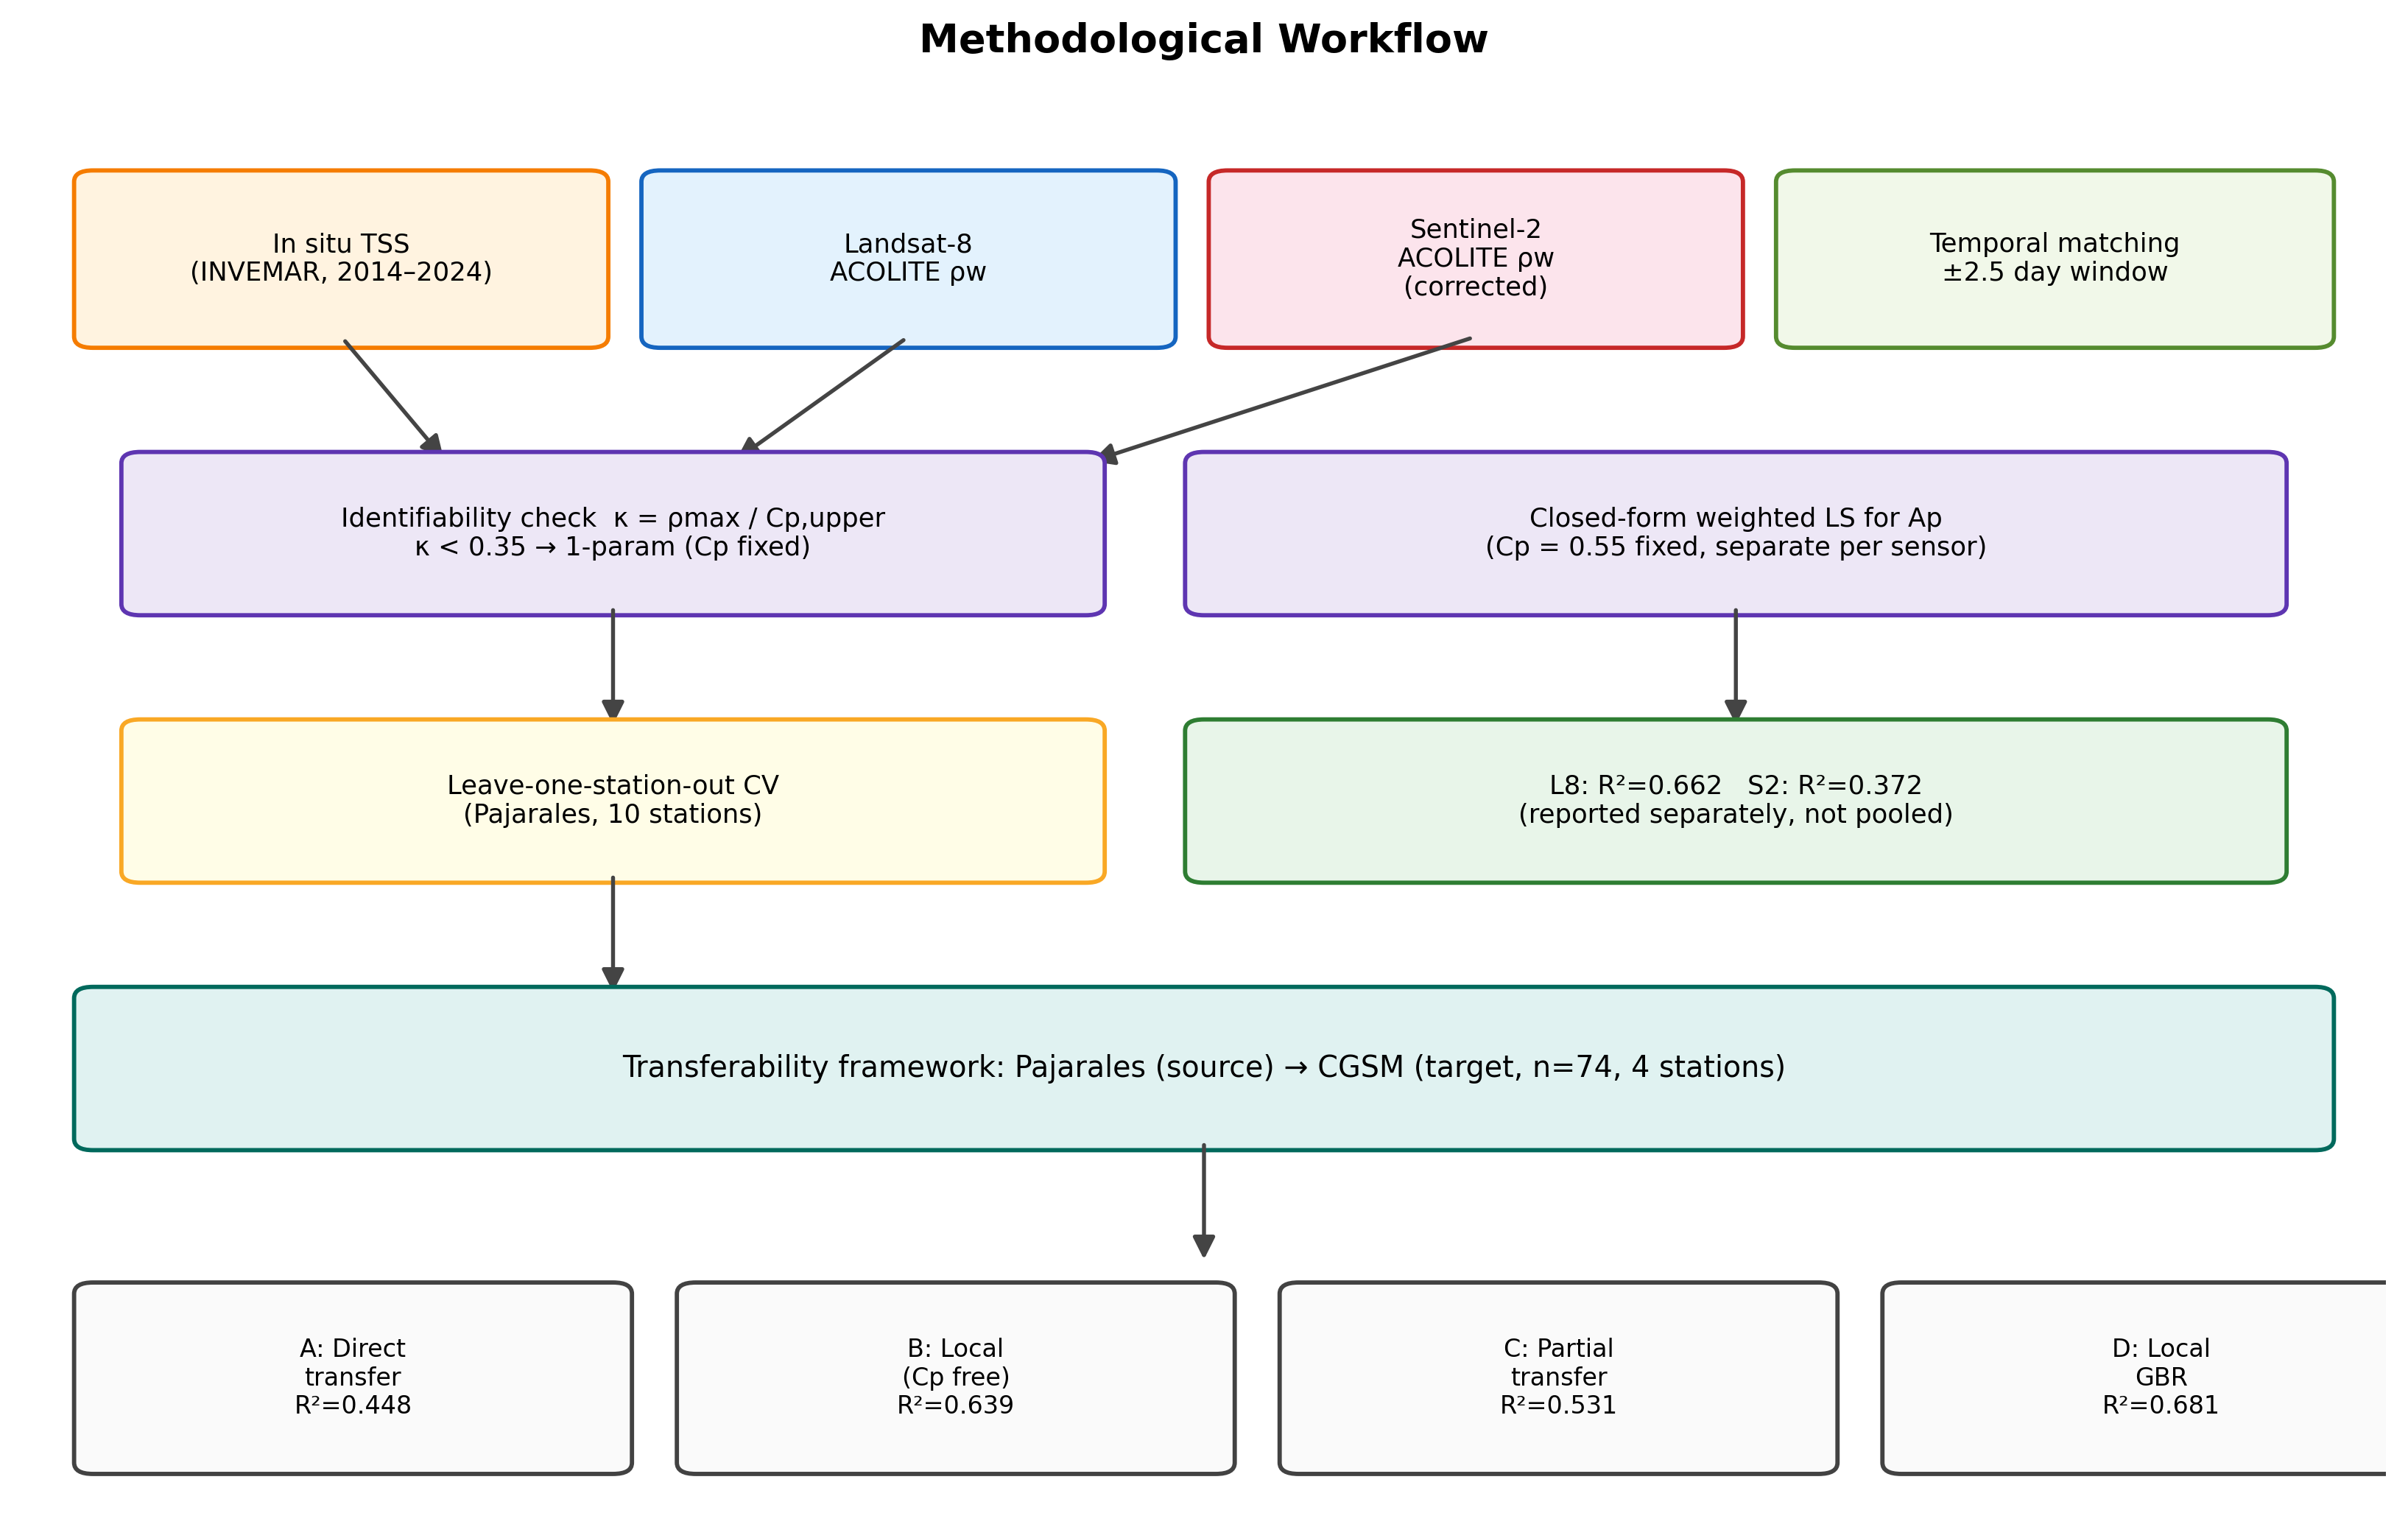
\includegraphics[width=1\textwidth,clip,trim=0 170 0 0]{images/methodology.png}
  \caption{Methodological conceptual diagram of sampling and analysis procedures.}
  \label{fig:methodology}
\end{figure}


\subsection{Satellite Image Acquisition and Temporal Matching}
\label{sec:matchup}
 
Each \textit{in situ} observation was paired with satellite imagery from Sentinel-2 or Landsat-8 acquired within a temporal window
centred on the sampling date. To determine the matchup window, a sensitivity analysis was conducted by progressively widening the maximum allowed lag from $\pm$0.5 up to $\pm$2.84~days (the largest lag present in the assembled matchup pool), evaluating leave-one-station-out cross-validated model performance at each threshold
(Section~\ref{sec:sensitivity}).

Leave-one-station-out $R^2$ peaked at a relatively tight window
($\pm$0.75--1.25~days, $R^2 = 0.735$, $n = 66$--67) and declined
gradually as the window widened further, reaching $R^2 = 0.662$ at the
full $\pm$2.84-day window used throughout this study ($n = 110$). This
indicates genuine temporal de-correlation of TSS dynamics at longer
lags, consistent with the temporal weighting scheme
(Equation~\ref{eq:weight}) being a necessary correction rather than a
formality: predictive skill is real but degrades smoothly, not
abruptly, as matchup age increases. The $\pm$2.5-day cutoff used
throughout this study was nonetheless retained, prioritising sample
size and station coverage over the small peak in cross-validated
$R^2$ available at a tighter window: at $\pm$0.75~days only 66 of the
240 available Pajarales matchups remain, with correspondingly thinner
per-station leave-one-out training folds, and several CGSM and
Sentinel-2 strata would fall below the $\text{MIN\_SAMPLES} = 5$
threshold required for a stable fit (Section~\ref{sec:identifiability}).
The exponential temporal weighting scheme (Equation~\ref{eq:weight})
is retained specifically to down-weight, rather than discard, the
more temporally distant matchups that this wider window admits. All
matchups in the final dataset fall within $\pm$2.84~days, the
practical ceiling of the assembled matchup pool rather than an
independently tested upper bound; performance at lags beyond this was
not evaluated, since no such matchups exist in the dataset.
 
Unlike traditional approaches relying exclusively on same-day matchups, this study implements a temporally weighted calibration framework to
explicitly account for the uncertainty introduced by non-coincident
observations. For each satellite--\textit{in situ} pair within the
selected window, a temporal weight $w_i$ was assigned as:
 
\begin{equation}
w_i = \exp\!\left(-\frac{|\Delta t_i|}{\tau}\right), \qquad \tau = 1\;\text{day}
\label{eq:weight}
\end{equation}
 
where $|\Delta t_i|$ is the absolute time difference in days and
$\tau = 1$~day is the decay constant, corresponding to a weight
half-life of $\ln(2) \approx 0.69$~days. This assigns maximum weight
($w = 1$) to same-day observations and progressively lower weights to
temporally distant matchups.

When multiple satellite images were available for the same
\textit{in situ} observation, all valid pairs were retained with their
corresponding weights, increasing effective sample size while preserving
temporal consistency. Surface reflectance values were extracted as the
median of a $3 \times 3$ pixel window
centred at the sampling location to minimise geolocation errors and sub-pixel variability. Outliers were
identified and removed using 5th--95th percentile filtering.
 
This temporally weighted strategy enables the integration of
non-synchronous observations while explicitly accounting for temporal
uncertainty \citep{Pahlevan2022, Espinoza2025}.


\subsubsection{Sentinel 2 dataset}

Sentinel-2 imagery was used, corresponding to tiles T18PWS and T18PWT, which cover the CGSM area. Images from both Sentinel-2A and Sentinel-2B satellites were selected, covering the period from their launch dates up to the end of 2024, with a cloud cover threshold of less than 30\%. All images were downloaded from the Copernicus Open Access Hub (https://scihub.copernicus.eu/) as Level-1C products, providing Top-Of-Atmosphere (TOA) reflectance values and orthorectified data. Sentinel-2, part of the Copernicus program, is designed to monitor terrestrial and coastal environments. It is equipped with the MultiSpectral Instrument (MSI), which captures high-resolution multispectral imagery suitable for detailed analyses of water bodies, vegetation, and land use dynamics.

Level-1C Sentinel-2 images offer a combined revisit time of 5 days due to the constellation of two satellites (Sentinel-2A and 2B). The imagery comprises 10 spectral bands within the visible and near-infrared (NIR) ranges, as well as 3 bands in the shortwave infrared (SWIR) range, including one specifically designed for detecting cirrus clouds. Spatial resolutions vary across bands: 10, 20, or 60 meters.

\subsubsection{Landsat 8 dataset}

Landsat 8 images were used, corresponding to path 009 and rows 052 and 053, selected from its launch date to the end of 2024, with a cloud cover of less than 30\%. Landsat 8, with its 16-day repeat cycle, captured the study area with two overlapping scenes every 7–9 days. The images were downloaded from the US Geological Survey (USGS) through the Global Visualization Viewer (http://glovis.usgs.gov/) and EarthExplorer (https://earthexplorer.usgs.gov/). The downloaded imagery includes five spectral bands in the visible and NIR range, three in the SWIR range (one dedicated to cirrus cloud detection), and a panchromatic band. All bands have a spatial resolution of 30 meters, except for the panchromatic band, which has 15 meters.

\subsection{Atmospheric Correction and Inter-Sensor Harmonization}
\label{sec:atmCorrection}

Satellite reflectance values used for total suspended solids (TSS) retrieval were derived from Landsat 8 (L8) and Sentinel-2 (S2) imagery following atmospheric correction. Atmospheric correction was performed using ACOLITE \cite{Vanhellemont2015, Vanhellemont2019}, a processor specifically designed for coastal and inland waters where adjacency effects, high turbidity, and complex aerosol conditions often limit the performance of conventional atmospheric correction methods.

The Dark Spectrum Fitting (DSF) algorithm was applied to convert top-of-atmosphere reflectance ($\rho_{\text{TOA}}$) into water-leaving reflectance ($\rho_{w}$). DSF estimates atmospheric path reflectance ($\rho_{\text{path}}$) from the darkest pixels in the scene without requiring predefined black-pixel regions, correcting for gaseous absorption, aerosol scattering, and sky reflectance. This approach is particularly suitable for optically complex and shallow estuarine environments, such as the Ciénaga Grande de Santa Marta.

An initial Sentinel-2 ACOLITE processing run was found, during internal review, to contain a residual atmospheric-correction artefact affecting a subset of acquisitions (Section~\ref{sec:disc_s2gap}); this was corrected and the corrected reflectance values are used throughout this study. Table~\ref{tab:spectral_bands} summarizes the central wavelengths and spatial resolutions of the spectral bands used for TSS estimation. Bands in the red and near-infrared regions were prioritized due to their sensitivity to suspended sediment concentrations.

Extreme values were filtered using a 5th--95th percentile range to reduce noise and outlier effects before model calibration. Landsat-8 reflectance was retained from the ACOLITE-processed product rather than from uncorrected Collection-2 Level-2 surface reflectance; a direct comparison (Section~\ref{sec:disc_acolite_vs_raw}) found ACOLITE retrievals to have approximately half the coefficient of variation of the uncorrected product at matched observations across all TSS levels, consistent with genuine noise suppression by the Dark Spectrum Fitting algorithm rather than an artefact of dynamic-range compression.

\begin{table}[h!]
\centering
\begin{tabular}{c|cc|cc}
\hline
\textbf{Band \#} & \multicolumn{2}{c|}{\textbf{Sentinel-2}} & 
\multicolumn{2}{c}{\textbf{Landsat-8}} \\
 & $\lambda$ (width) & SR & $\lambda$ (width) & SR \\
\hline
1 & 443 (20) & 60 & 443 (20) & 30 \\
2 & *490 (65) & 10 & *482 (60) & 30 \\
3 & 560 (35) & 10 & 562 (60) & 30 \\
4 & *665 (30) & 10 & *655 (30) & 30 \\
5 & *705 (15) & 20 & *865 (30) & 30 \\
6 & *740 (15) & 20 & *1609 (80) & 30 \\
7 & *783 (20) & 20 & 2204 (180) & 30 \\
8 & *842 (115) & 10 & 590 (180) & 15 \\
8a & 865 (20) & 20 & -- & -- \\
9 & 945 (20) & 60 & 1374 (20) & 30 \\
10 & 1380 (30) & 60 & -- & -- \\
11 & 1610 (90) & 20 & -- & -- \\
12 & 2190 (180) & 20 & -- & -- \\
\hline
\end{tabular}
\caption{Central wavelength ($\lambda$) and spatial resolution (SR) of the spectral bands used from Sentinel-2 and Landsat-8.}
\label{tab:spectral_bands}
\end{table}

% ── TSS RETRIEVAL MODEL ──────────────────────────────────────────
\subsection{TSS Retrieval Model}
\label{sec:tss_models}
 
\subsubsection{Model Formulation}
 
Match-ups between atmospherically corrected satellite reflectance and
\textit{in situ} TSS measurements were constructed using a temporal
window of $\pm$2.5~days. The semi-analytical model of
\citet{NECHAD2010854} was used as the primary TSS retrieval model:
 
\begin{equation}
\text{TSS} = A_p \cdot \frac{\rho_w}{1 - (\rho_w / C_p)}
\label{eq:nechad}
\end{equation}

where $\rho_w$ is the atmospherically corrected water-leaving
reflectance, $A_p~(mg/L$) is an amplitude coefficient encoding
backscattering efficiency, and $C_p$ is the saturation reflectance
asymptote, physically bounded between approximately 0.10 and 0.55 for
the red band \citep{NECHAD2010854}. A power-law model
($\text{TSS} = a\,\rho^b$) was also evaluated as a comparison
benchmark but not adopted as the primary retrieval model.
 
 
\subsubsection{Parameter Identifiability Assessment}
\label{sec:identifiability}
 
Reliable estimation of both $A_p$ and $C_p$ from data requires that
observed reflectances span sufficient curvature of
Equation~(\ref{eq:nechad}). We define the identifiability ratio:
 
\begin{equation}
\kappa = \frac{\rho_{\max}}{C_{p,\text{upper}}}
\label{eq:kappa}
\end{equation}
 
where $C_{p,\text{upper}}$ is the upper physical bound for the relevant
spectral band (0.20 for blue $\sim$490~nm; 0.55 for red $\sim$665~nm;
0.60 for NIR $\sim$865~nm). When $\kappa < 0.35$, the data lie on the
near-linear segment of the Nechad curve and $C_p$ cannot be
independently estimated; any large value of $C_p$ yields virtually
identical fit quality, causing gradient-based optimisers to drift to
physically meaningless values that span many orders of magnitude.
When $\kappa \geq 0.35$, sufficient curvature exists for free
two-parameter fitting in principle; in practice, however, even when
$\kappa \geq 0.35$ the fitted $C_p$ was found to converge to
$C_{p,\text{upper}}$ regardless of optimiser initialisation for both
sensors at Pajarales (Section~\ref{sec:results_calibration}), so both
sensors are reported as effectively one-parameter fits with
$C_p = C_{p,\text{upper}}$ fixed. Following this criterion, all
retrieval in this study uses a single band, $\rho_{665}$ (red, B4), for
which $\kappa$ is computed once per sensor from that sensor's full
Pajarales matchup set: $\kappa_{\text{L8}} = 0.343$ and
$\kappa_{\text{S2}} = 0.452$ (corrected reflectance;
Section~\ref{sec:disc_s2gap}).
 
When $\kappa < 0.35$ (\textbf{one-parameter mode}), $C_p$ is fixed to
the band's physical upper bound, $C_{p,\text{upper}}$, and $A_p$ is
estimated analytically via the closed-form weighted least-squares
solution:
 
\begin{equation}
\hat{A}_p = \frac{\displaystyle\sum_{i} w_i\,\text{TSS}_i\,\varphi_i}
{\displaystyle\sum_{i} w_i\,\varphi_i^2},
\qquad
\varphi_i = \frac{\rho_i}{1 - \rho_i / C_p}
\label{eq:ap_closed}
\end{equation}
 
where $w_i$ are the temporal weights from Equation~(\ref{eq:weight}).
This is the analytically exact maximum-likelihood estimator for $A_p$
given known $C_p$. When $\kappa \geq 0.35$, both $A_p$ and $C_p$ are
first estimated by non-linear weighted least squares, multi-start
initialised over a grid of starting values for $C_p \in
[C_{p,\text{lower}},\, C_{p,\text{upper}}]$; if the optimised $C_p$
converges to $C_{p,\text{upper}}$ regardless of starting value, the
fit is reported and treated as one-parameter (Equation~\ref{eq:ap_closed})
for all downstream cross-validation, since a boundary-converged
two-parameter fit carries no additional information over the
closed-form solution and is less numerically stable when refit on
leave-one-station-out training folds.
 
For both fitting modes, points within 10\% of the active $C_p$ are
excluded from the fitting step only, to prevent the small number of
near-asymptote observations from dominating the weighted solution
through their disproportionately large $\varphi_i$. These points
remain in the dataset and are still predicted and scored when
performance metrics are computed.
 
Within each sensor's fitting mode, $A_p$ is estimated separately for
Landsat-8 and Sentinel-2, rather than pooled across sensors. A pooled
single-$A_p$ fit across both sensors was evaluated and found to
underperform either single-sensor fit (Section~\ref{sec:disc_pooling}),
consistent with a persistent inter-sensor reflectance offset described
below; OWT classification, based on the relative magnitude of the
blue ($\rho_{490}$), green ($\rho_{560}$), and red ($\rho_{665}$)
bands, is retained as a descriptive water-type diagnostic
(Section~\ref{sec:results_calibration}) but is not used to stratify
the fitted Nechad parameters, which are reported per sensor only.
 
 
\subsubsection{Cross-Validation Strategy}
\label{sec:cv}
 
Model performance is reported from leave-one-station-out
cross-validation rather than random $k$-fold CV. For each monitoring
station, parameters are re-estimated using all data from the
\emph{other} stations and applied to the held-out station only; this is
repeated once per station and predictions are pooled across all
held-out folds for the reported metrics. This procedure tests genuine
spatial generalisation to unseen locations, rather than interpolation
within already-sampled sites, and avoids both the autocorrelation
leakage of random fold assignment and the circularity of stratifying by
a target-derived category. In-sample (training-set) statistics are
reported separately and are not used as primary performance indicators.

\subsubsection{Performance Metrics}
\label{sec:metrics}
 
Model performance was evaluated using four metrics computed between
cross-validated predictions and \textit{in situ} TSS measurements:
 
\begin{align}
R^2         &= 1 - \frac{\displaystyle\sum_i (\text{TSS}_i - \hat{y}_i)^2}
                        {\displaystyle\sum_i (\text{TSS}_i - \overline{\text{TSS}})^2}
\label{eq:r2}\\[6pt]
\text{RMSE} &= \sqrt{\frac{1}{n}\sum_i (\text{TSS}_i - \hat{y}_i)^2}
\label{eq:rmse}\\[6pt]
\text{Bias} &= \frac{1}{n}\sum_i (\hat{y}_i - \text{TSS}_i)
\label{eq:bias}\\[6pt]
\text{MAPE} &= \frac{100}{n}\sum_i
              \left|\frac{\text{TSS}_i - \hat{y}_i}{\text{TSS}_i}\right|
\label{eq:mape}
\end{align}
 
 
% ── SENTINEL-1 ───────────────────────────────────────────────────
\subsection{Water Surface Area Dynamics from Sentinel-1}
\label{sec:s1}
 
To complement the optical TSS analysis, monthly water surface extent
within the CGSM was derived from Sentinel-1 (S1) Synthetic Aperture
Radar (SAR) imagery. Radar data were selected because they are
unaffected by cloud cover, ensuring a continuous record even during the
rainy season when optical sensors have limited availability.
 
Sentinel-1 Ground Range Detected (GRD) products acquired in
Interferometric Wide (IW) swath mode were used, considering only
descending-orbit scenes with VV polarisation and a spatial resolution
of approximately 10~m. Data were accessed and processed within Google
Earth Engine, which provides radiometrically calibrated and
terrain-corrected backscatter coefficients ($\sigma^0$, in dB).
 
Water surfaces were identified by classifying pixels with VV backscatter
below a fixed threshold of $-17$~dB as water, a criterion validated for
coastal lagoon and wetland environments. For each month, the total water
surface area (km$^2$) was computed by summing the area of water-classified
pixels within the CGSM boundary polygon (derived from the INVEMAR water
mask shapefile). Monthly and annual time series were computed for the
period 2015--2025.

The S1-derived water surface area time series was temporally aligned
with \textit{in situ} TSS observations and the Oceanic Ni\~{n}o Index
(ONI, NOAA CPC) to investigate hydro-sedimentary and hydroclimatic
relationships. Statistical analyses comprised Pearson and Spearman
correlations and Mann-Kendall trend tests to characterise the
direction, magnitude, and significance of long-term changes and
cross-variable associations.
 
 
% ── TRANSFERABILITY FRAMEWORK ─────────────────────────────────────
\subsection{Transferability Framework}
\label{sec:transfer}
 
The limited number of satellite--\textit{in situ} matchups in the CGSM
($n = 74$) and their concentration in a narrow reflectance range
($\rho_{B4} = 0.012$--$0.071$; $\kappa = 0.13$) motivated a systematic
multi-scenario transferability assessment. Four scenarios were
evaluated using leave-one-station-out cross-validation on the CGSM
dataset (four monitoring stations):
 
\begin{itemize}
    \item \textbf{Scenario~A — Direct transfer:} the Pajarales-calibrated
          Landsat-8 model ($A_p = 1476.2$, $C_p = C_{p,\text{upper}} = 0.55$;
          Section~\ref{sec:results_calibration}) applied to CGSM
          reflectances unchanged, with no local adjustment at all and no
          leave-one-station-out refitting (the model never sees CGSM
          data). Establishes a lower-bound, zero-local-data baseline.
 
    \item \textbf{Scenario~B — Local NECHAD ($C_p$ free):} both $A_p$
          and $C_p$ fitted directly on CGSM data, free two-parameter fit
          (bounded $[0.10, C_{p,\text{upper}}]$), re-estimated for each
          held-out station from the other three. Full local
          recalibration.
 
    \item \textbf{Scenario~C — Partial transfer (proposed):} $C_p$
          fixed at $C_{p,\text{upper}}$ (the same anchor as Pajarales);
          $A_p$ refitted on CGSM data for each held-out station from the
          other three. A single $A_p$ is fit across all CGSM data, since
          the sample is too small to support the same optical-water-type
          stratification used for Pajarales. Proposed as a lower-data
          operational strategy for new sub-basins.
 
    \item \textbf{Scenario~D — Local GBR:} Gradient Boosting
          Regressor trained on the four raw reflectance bands
          ($\rho_{490}$, $\rho_{560}$, $\rho_{665}$, $\rho_{865}$),
          re-estimated for each held-out station from the other three
          using CGSM data only. Provides a non-physical performance
          ceiling.
\end{itemize}
 
The physical rationale for Scenario~C is that $C_p$ encodes the
saturation reflectance determined by particle optical properties --
primarily size distribution and composition, which are expected to be
comparable between Pajarales and the CGSM given their shared Magdalena
River sediment provenance \citep{NECHAD2010854}. In contrast, $A_p$ scales
the local reflectance--TSS relationship and may differ between sites.
As shown in Section~\ref{sec:results_transfer}, this physical rationale
does not translate into an accuracy advantage at this site: CGSM's own
reflectance range lies almost entirely below 10\% of $C_{p,\text{upper}}$,
so fixing $C_p$ there leaves the curve close to linear over the
observed domain and removes the curvature information that a locally
free $C_p$ (Scenario~B) can exploit.
 
Before the transferability analysis, reflectance domain overlap was
quantified as the fraction of $\rho_{B4}$ observations at each site
falling within the reflectance range of the other, to diagnose whether
Scenario~A involves extrapolation.

%%%%%%%%%%%%%%%%%%%%%%%%%%%%%%%%%%%%%%%%%%
\section{Results}

\subsection{Dataset Characterisation and Identifiability Diagnostics}
\label{sec:sensitivity}
The Pajarales calibration dataset comprised 130 Sentinel-2 and
110~Landsat-8 matchups ($n = 240$, 2015--2026). The CGSM validation
dataset comprised 74~Landsat-8 matchups ($n = 74$, 2015--2024).
Landsat-8 exhibited a stronger reflectance--TSS
correlation at Pajarales ($r = 0.847$) than Sentinel-2 ($r = 0.622$,
after correction of the atmospheric-correction artefact identified in
Section~\ref{sec:disc_s2gap}; the uncorrected value was $r = 0.118$),
both on the red band ($\rho_{665}$, B4). $\kappa$ is computed once per
sensor from the full Pajarales matchup set for that sensor
(Section~\ref{sec:identifiability}): Landsat-8 ($\kappa = 0.343$) falls
below the $\kappa = 0.35$ threshold and uses one-parameter fitting with
$C_p$ fixed; Sentinel-2 ($\kappa = 0.452$) nominally exceeds the
threshold, but its two-parameter fit converges to $C_p = C_{p,\text{upper}}$
regardless of optimiser initialisation and is therefore also treated as
one-parameter (Section~\ref{sec:identifiability}). CGSM data
($\kappa_{B4} = 0.13$) fall below the threshold, requiring
one-parameter fitting with $C_p$ fixed.
 
\begin{table}[ht]
\centering
\caption{Reflectance range and identifiability ratio ($\kappa$) per
sensor on the red band ($\rho_{665}$, B4) -- the only band used for
TSS retrieval in this study. $r$ denotes the Pearson correlation with
\textit{in situ} TSS. $\kappa < 0.35$: one-parameter mode
($C_p$ fixed); $\kappa \geq 0.35$ nominal, but boundary-converged and
treated as one-parameter in practice (Sentinel-2, see text).}
\label{tab:identifiability}
\small
\begin{tabular}{llccccc}
\toprule
Site & Sensor & Band & $\lambda$ (nm) & $\rho_{\max}$ & $\kappa$ & Mode ($r$) \\
\midrule
Pajarales & L8 & B4 & 665 & 0.189 & 0.343 & 1-param (0.847) \\
Pajarales & S2 & B4 & 665 & 0.249 & 0.452 & 1-param$^*$ (0.622) \\
CGSM      & L8 & B4 & 655 & 0.071 & 0.13  & 1-param (0.775)  \\
\bottomrule
\end{tabular}
\end{table}
{\small $^*$Nominally two-parameter ($\kappa \geq 0.35$); fitted $C_p$
converges to $C_{p,\text{upper}}$ at every optimiser initialisation
tested and is reported as one-parameter for this reason
(Section~\ref{sec:identifiability}).}
 
Figure~\ref{fig:sensitivity} shows leave-one-station-out CV~$R^2$ as a
function of the maximum temporal lag threshold. Performance peaks at a
tight window ($\pm$0.75--1.25~days, $R^2 = 0.735$) and declines
gradually as the window widens, reaching $R^2 = 0.662$ at the
$\pm$2.84-day ceiling of the assembled matchup pool -- the window used
throughout this study. This pattern motivates the temporal weighting
scheme (Equation~\ref{eq:weight}) and the choice to prioritise sample
size and per-station fold stability over the smaller, tighter-window
peak (Section~\ref{sec:matchup}).
 
\begin{figure}[h!]
    \centering
    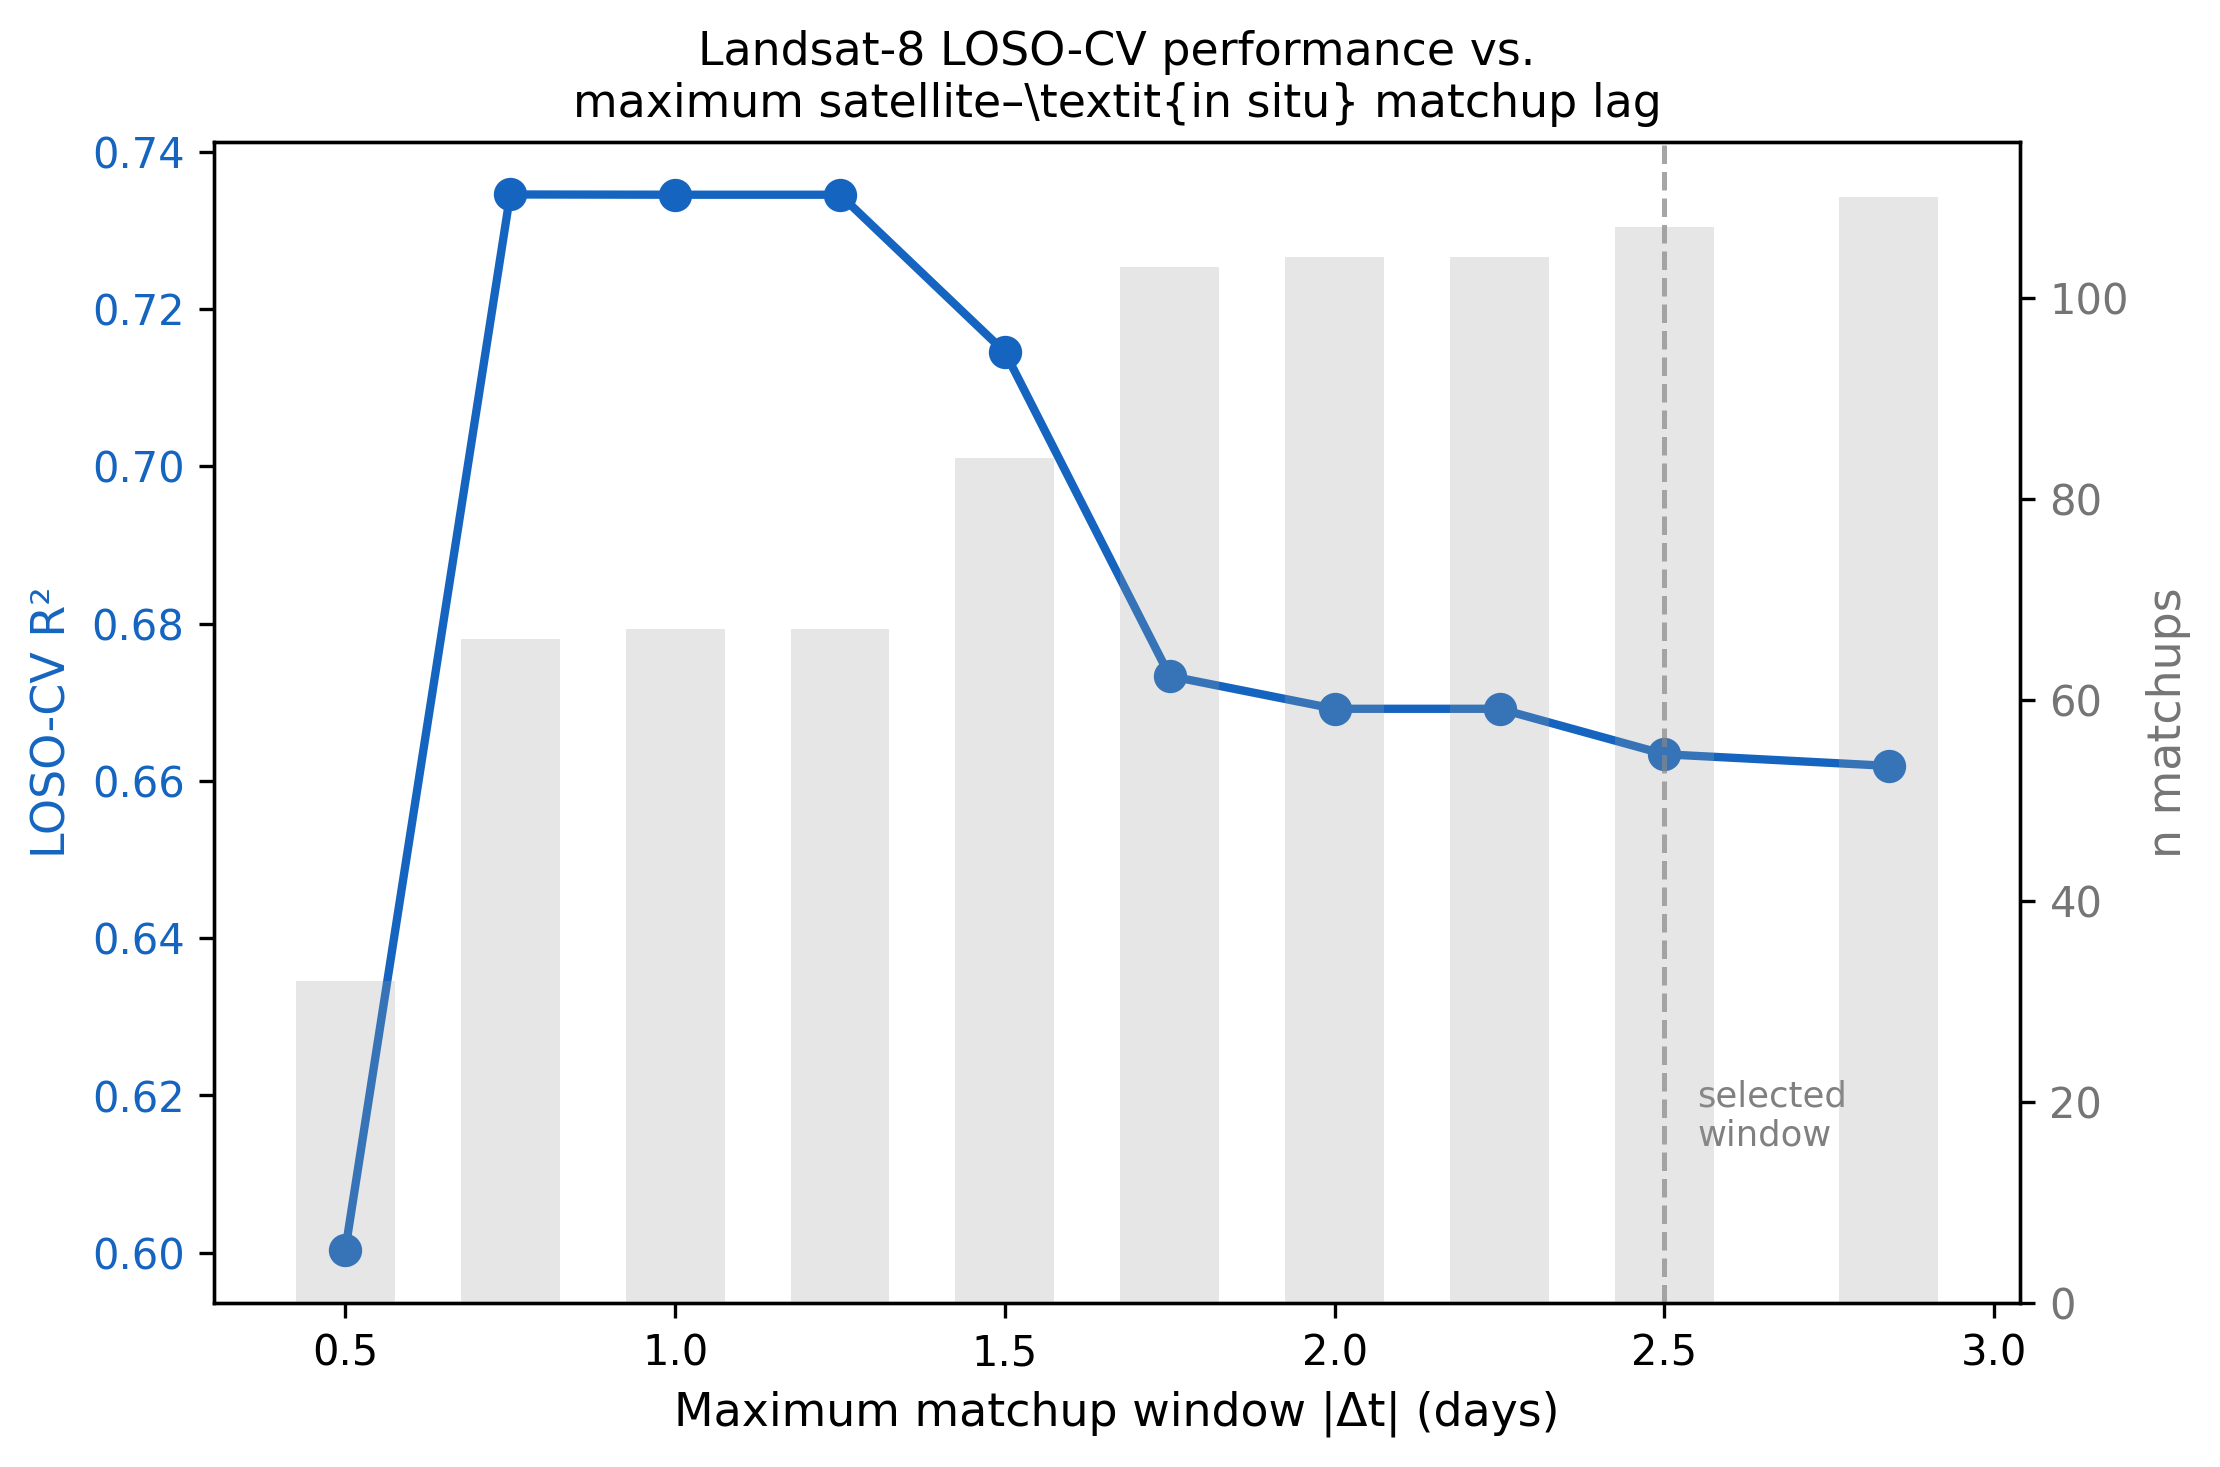
\includegraphics[width=0.80\linewidth]{images/fig1_temporal_sensitivity.png}
    \caption{Leave-one-station-out CV~$R^2$ (left axis, line) and
    matchup count (right axis, bars) as a function of maximum temporal
    matchup window (Pajarales L8, B4, fixed $C_p$ NECHAD). Performance
    peaks near $\pm$1~day and declines gradually as more, more
    temporally distant matchups are admitted, reaching $R^2 = 0.662$
    at the $\pm$2.84-day window used throughout this study (dashed
    line).}
    \label{fig:sensitivity}
\end{figure}

Figure~\ref{fig:identifiability} shows reflectance domain overlap and identifiability ratios. CGSM's reflectance domain occupies only the lower portion of the Pajarales range: the CGSM maximum ($\rho_{B4} = 0.071$) corresponds to approximately the 35th percentile of the Pajarales Landsat-8 distribution, confirming that Scenario~A (Section~\ref{sec:transfer}) constitutes genuine extrapolation beyond, not merely a smaller sample within, the calibration domain.
 
\begin{figure}[h!]
    \centering
    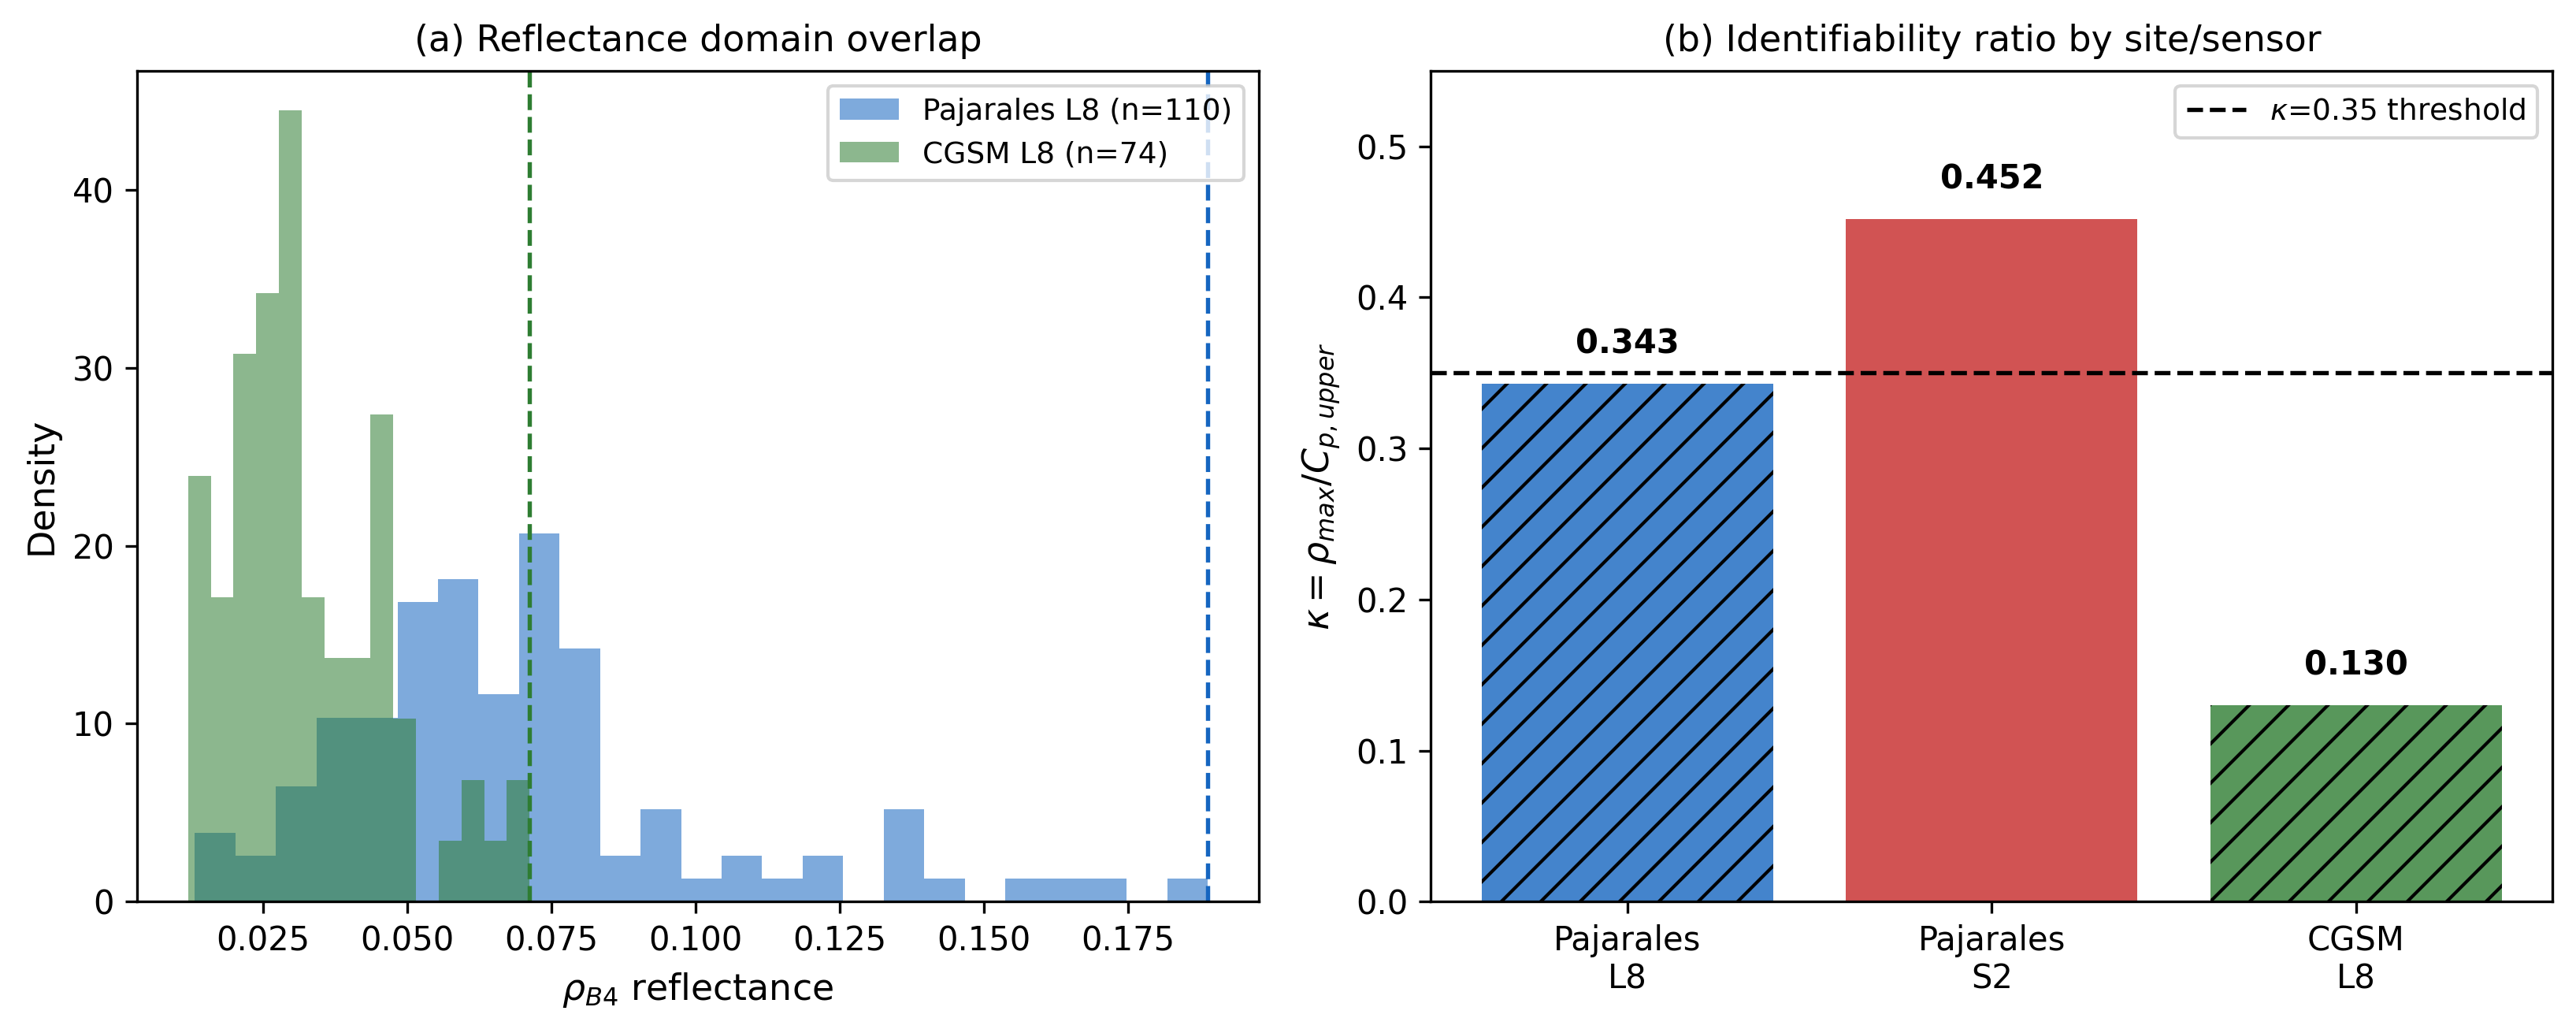
\includegraphics[width=0.95\linewidth]{images/fig5_domain_identifiability.png}
    \caption{Left: Reflectance domain overlap ($\rho_{B4}$,
    $\sim$665~nm) between Pajarales and CGSM. CGSM's range sits within
    the lower portion of the Pajarales distribution. Right: Identifiability
    ratio $\kappa$ per sensor--site--band. Hatched bars fall below
    $\kappa = 0.35$ and require one-parameter mode.}
    \label{fig:identifiability}
\end{figure}
 
 
% ── §3.2 ────────────────────────────────────────────────────────
\subsection{Pajarales Model Calibration and Cross-Validation}
\label{sec:results_calibration}
 
Landsat-8 and Sentinel-2 are calibrated and reported as separate
single-sensor models throughout (Section~\ref{sec:identifiability}); a
pooled single-$A_p$ fit across both sensors was tested and found to
underperform either sensor alone (Section~\ref{sec:disc_pooling}) and
is not used as the primary retrieval.
 
Table~\ref{tab:pajarales_cv} presents in-sample and leave-one-station-out
cross-validated performance for each sensor. For Landsat-8 ($n=110$),
the model achieves in-sample $R^2 = 0.693$ (RMSE $= 60.3$~mg/L) and
leave-one-station-out $R^2 = 0.662$ (RMSE $= 63.3$~mg/L). For
Sentinel-2 ($n=130$, corrected reflectance), the model achieves
in-sample $R^2 = 0.419$ (RMSE $= 56.6$~mg/L) and leave-one-station-out
$R^2 = 0.372$ (RMSE $= 73.2$~mg/L, $n=56$ scored observations from
stations with usable coordinates). For both sensors, $A_p$ is fitted
once per sensor on the full Pajarales matchup set, with $C_p$ fixed at
$C_{p,\text{upper}} = 0.55$ (Landsat-8: $A_p = 1476.2$; Sentinel-2:
$A_p = 533.2$); the leave-one-station-out figures refit $A_p$ on each
training fold using the same fixed $C_p$.
 
\begin{table}[ht]
\centering
\caption{TSS retrieval performance for Pajarales, by sensor
(Landsat-8, $n=110$; Sentinel-2, $n=130$, corrected reflectance), one-
parameter NECHAD ($C_p = C_{p,\text{upper}} = 0.55$ fixed,
Section~\ref{sec:identifiability}). Leave-one-station-out CV is the
primary reported metric; in-sample is shown for reference only.}
\label{tab:pajarales_cv}
\small
\begin{tabular}{p{4.6cm}cccc}
\toprule
Sensor / Evaluation & $A_p$ & $R^2$ & RMSE (mg\,L$^{-1}$) & $n$ \\
\midrule
Landsat-8, in-sample (reference)        & 1476.2 & 0.693 & 60.3 & 110 \\
Landsat-8, leave-one-station-out (primary) & 1476.2 & 0.662 & 63.3 & 110 \\
\addlinespace
Sentinel-2, in-sample (reference)       & 533.2  & 0.419 & 56.6 & 130 \\
Sentinel-2, leave-one-station-out (primary) & 533.2 & 0.372 & 73.2 & 56 \\
\bottomrule
\end{tabular}
\end{table}
 
Figure~\ref{fig:calib_cv} shows observed vs.\ predicted TSS for both
sensors under leave-one-station-out cross-validation, the figure of
record for each model's predictive performance.
 
\begin{figure}[h!]
    \centering
    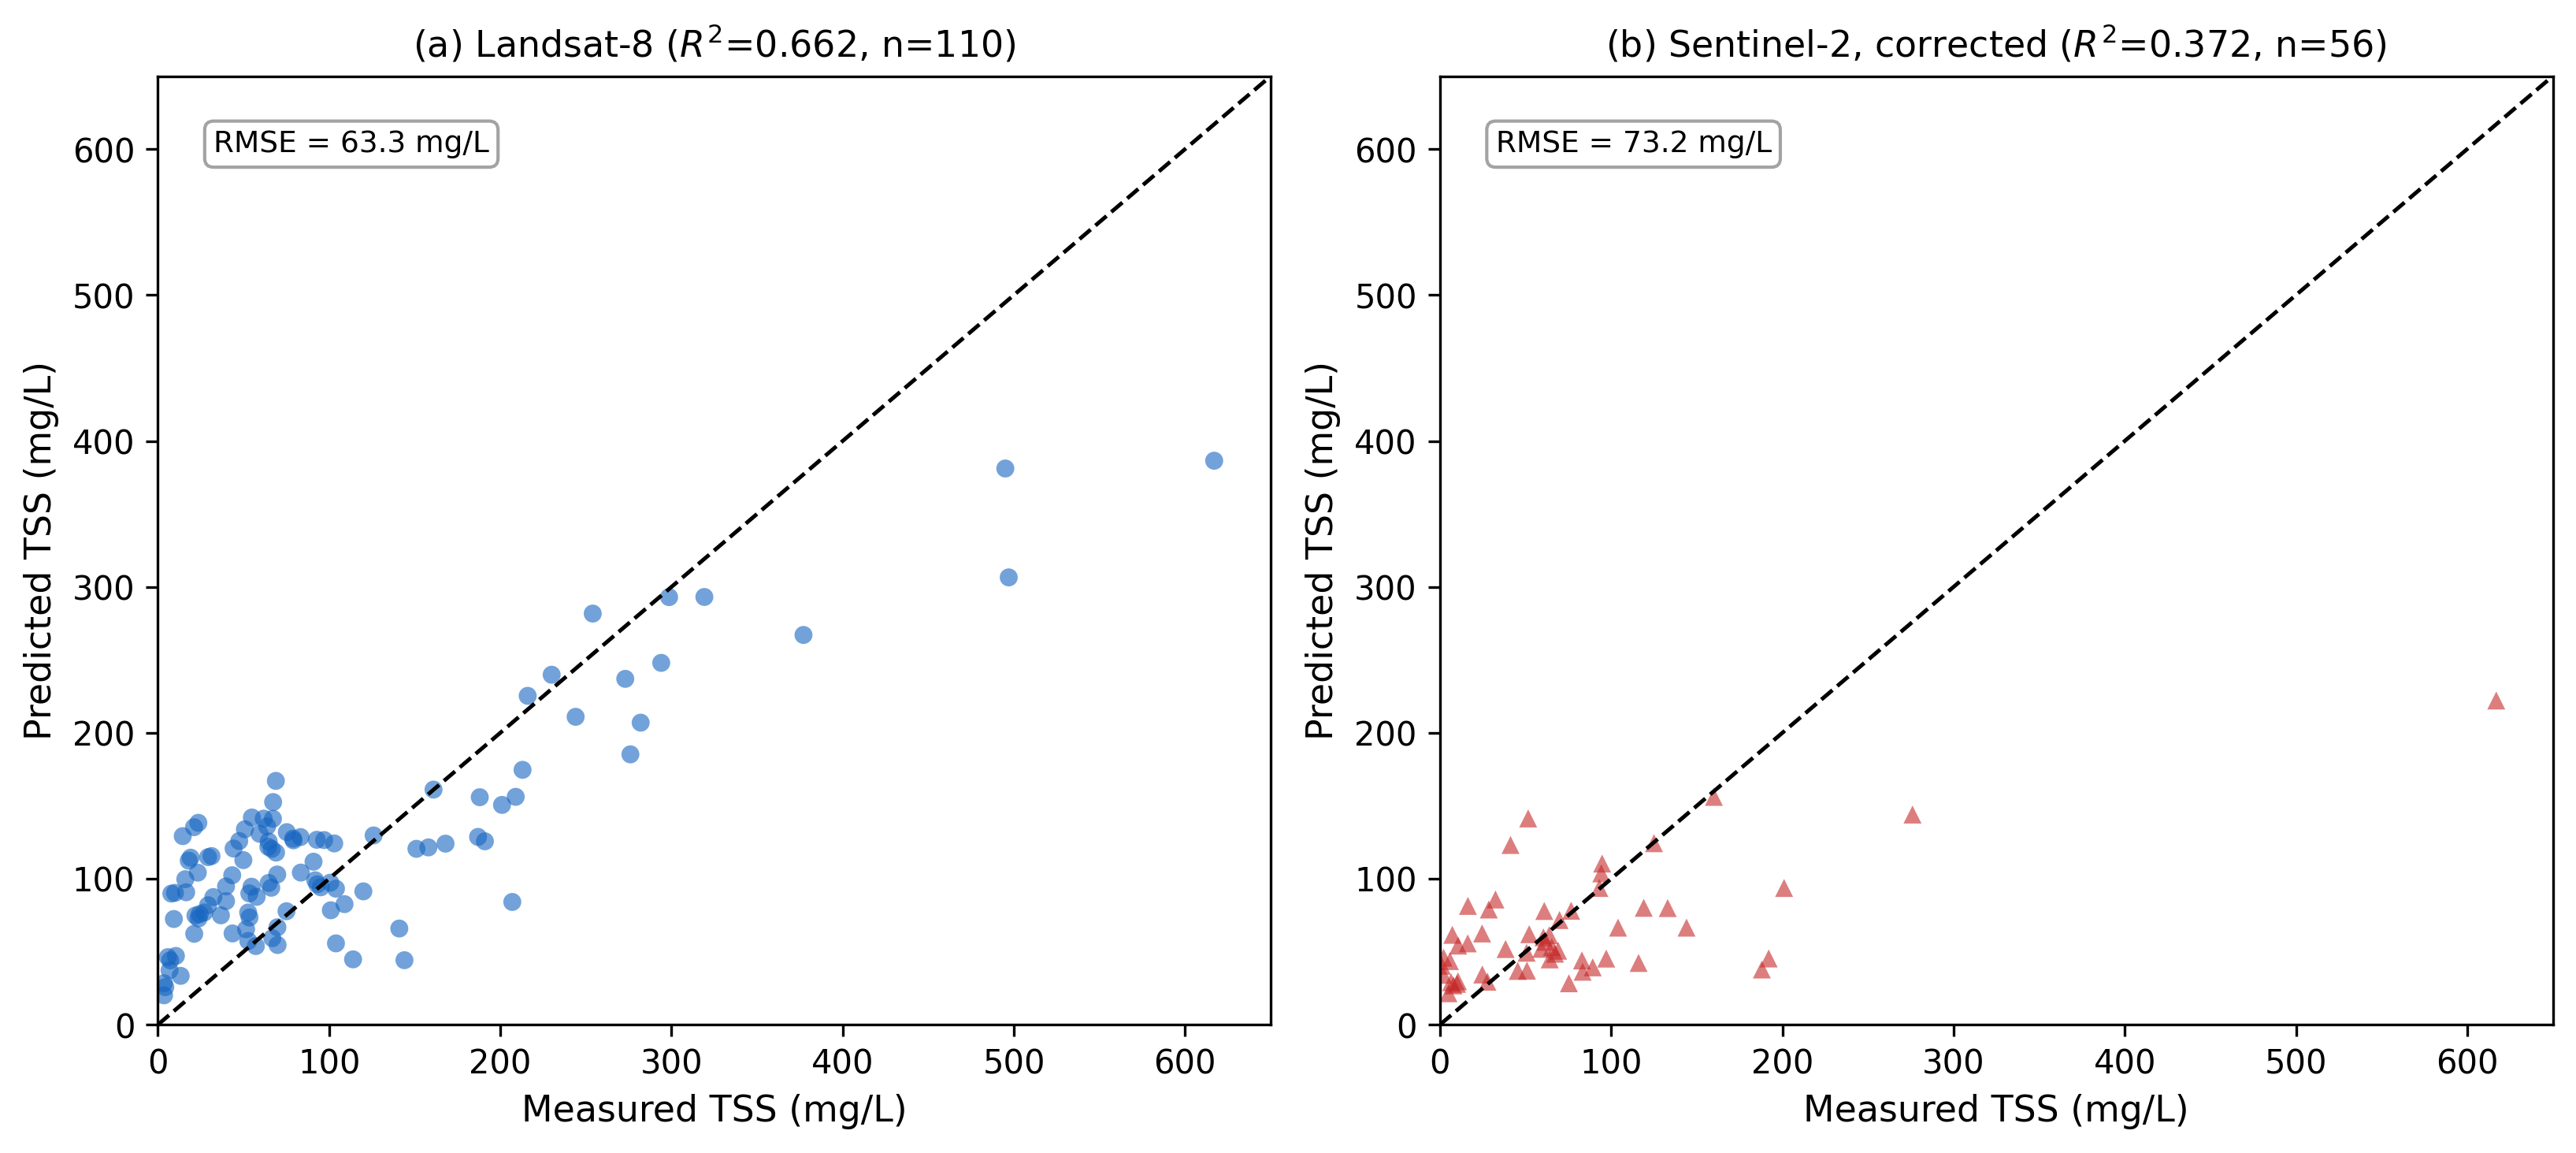
\includegraphics[width=0.95\linewidth]{images/fig2_pajarales_cv_scatter.png}
    \caption{Observed vs.\ predicted TSS at Pajarales under
    leave-one-station-out cross-validation. Left: Landsat-8
    ($R^2 = 0.662$, $n=110$). Right: Sentinel-2, corrected reflectance
    ($R^2 = 0.372$, $n=56$) -- the primary reported performance metric
    for each sensor, since it tests generalisation to monitoring
    stations unseen during fitting. Dashed line: 1:1 relationship.}
    \label{fig:calib_cv}
\end{figure}

 
 
% ── §3.4 ────────────────────────────────────────────────────────
\subsection{Spatial Distribution of TSS (2015--2024)}
\label{sec:results_spatial}

A total of 240 valid satellite--\textit{in situ} matchups were obtained
at Pajarales (130~Sentinel-2, 110~Landsat-8) and 74~at the CGSM.
Image availability increased substantially after 2016. Annual matchup
counts ranged from 8 (2015, dry-season concentrated) to 46 (2024).

Annual median TSS maps were generated by applying the calibrated, per-sensor NECHAD model to the full multi-sensor satellite archive (2013–2024) and should be interpreted as model-derived products rather than direct in situ measurements. Because Sentinel-2 retrieval performance is markedly weaker than Landsat-8 (Table~\ref{tab:pajarales_cv}), Sentinel-2-derived pixels in these composites should be interpreted qualitatively, as a spatial/temporal coverage supplement to the quantitatively stronger Landsat-8 product, rather than with equivalent confidence (Section~\ref{sec:disc_s2gap}).
Figure~\ref{fig:mosaico} illustrates the spatial distribution of annual median TSS across the Pajarales sector and the central CGSM for each year of the record. The persistent spatial contrast between the Pajarales Complex (annual medians 20–60 $mg/L$) and the CGSM main body (5–15 $mg/L$) is visible in every year without exception, providing spatial confirmation of the reflectance domain contrast reported in
Table~\ref{tab:identifiability} ($\rho_{B4}$ up to 0.19 vs 0.07). Elevated TSS concentrations are recurrently observed in the western Pajarales channels proximal to the Magdalena River inputs. Interannual variability in Pajarales is evident, with more intense warm tones visible in 2015–2016 and 2022–2023, broadly consistent with the matchup-derived annual anomalies discussed in
Section~\ref{sec:results_temporal}. Red circles indicate station-years where annual median TSS exceeded the Colombian water quality reference threshold of 150 $mg/L$ (Resolución 883 de 2018).

\begin{figure}[htbp]
    \centering
    \includegraphics[
        width=0.85\textwidth,
        clip,
        trim=0 20 0 50
    ]{images/TSS_promedio_anual_mosaico_CGSM.png}
    \caption{Annual median satellite-derived TSS (mg /L) across the
    Ciénaga Grande de Santa Marta and Pajarales Complex (2013--2024), derived
    by applying the calibrated per-sensor NECHAD model to the full
    Landsat-8 and Sentinel-2 archive.}
    \label{fig:mosaico}
\end{figure}
 
 
% ── §3.5 ────────────────────────────────────────────────────────
\subsection{Temporal Dynamics and Seasonal Variability}
\label{sec:results_temporal}
 
Dry-season observations (January--April) at Pajarales had a median of
$75.3~mg/L$ compared with $29.3~mg/L$ during the wet season
(July--November; Kruskal--Wallis $p < 0.001$). No significant seasonal
differentiation was detected at the CGSM ($p = 0.80$). Monthly
climatology at Pajarales peaks in March--April
($\sim 90--95~mg/L$) and reaches minimum values in November
($\sim 9~mg/L$), consistent with wind-driven resuspension during
the northeast trade wind season.
 
Annual median TSS was highest in 2015--2016 and lowest in 2024
($18~mg/L$; $n = 21$). The 2015 estimate
(median $296~mg/L$) should be treated cautiously as it is based on only $n = 8$ observations concentrated in the dry season.
 
\begin{figure}[h!]
    \centering
    \includegraphics[width=0.95\linewidth]{images/fig4_monthly_climatology.png}
    \caption{Monthly TSS climatology from \textit{in situ} matchup
    data. Top: Pajarales ($n = 240$, L8 + S2) --- significant
    dry-season peak (March--April). Bottom: CGSM ($n = 74$, L8) ---
    flat seasonal pattern (KW $p = 0.80$). Colours denote season.}
    \label{fig:climatology}
\end{figure}
 
\begin{figure}[h!]
    \centering
    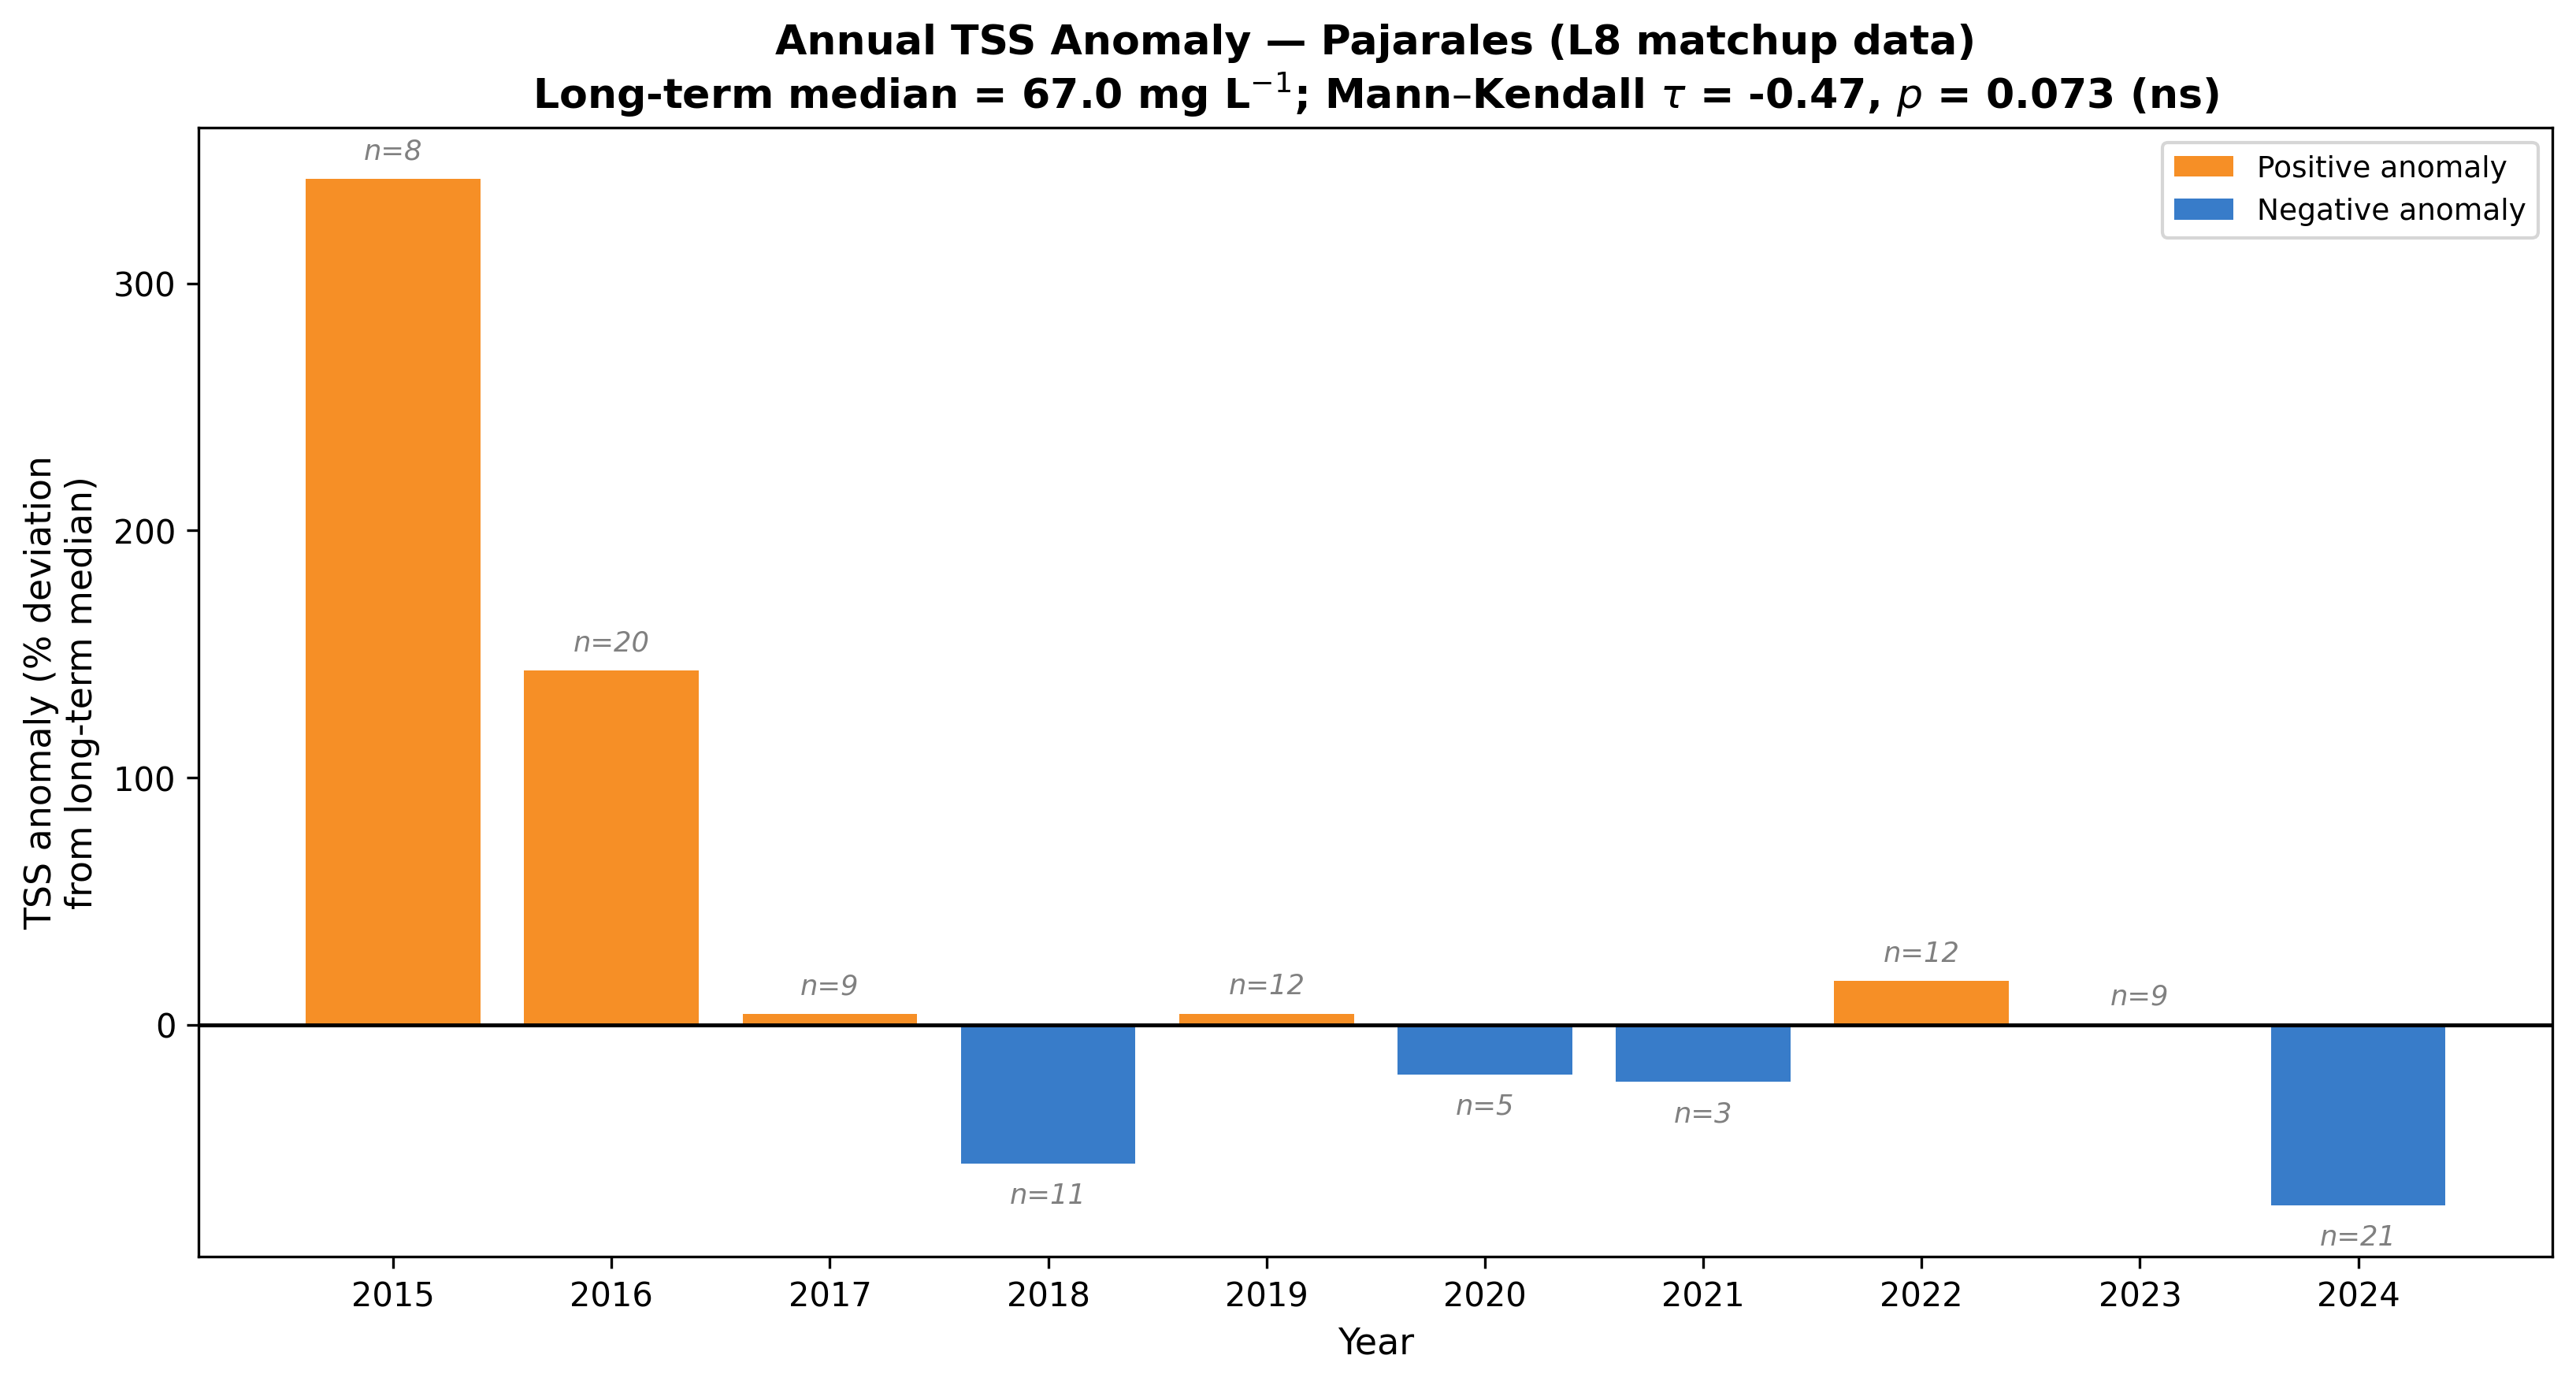
\includegraphics[width=0.95\linewidth]{images/fig6_annual_anomalies.png}
    \caption{Annual TSS anomaly (\% deviation from long-term median)
    at Pajarales (L8 matchup data, 2015--2024). Numbers indicate
    sample size per year. Mann--Kendall $\tau = -0.47$
    ($p = 0.073$, non-significant).}
    \label{fig:anomalies}
\end{figure}
 
 
% ── §3.6 ────────────────────────────────────────────────────────
\subsection{Transferability Analysis: Pajarales to CGSM}
\label{sec:results_transfer}
 
Table~\ref{tab:transferability} presents leave-one-station-out
cross-validated performance for the four transferability scenarios,
using the Landsat-8 calibration as the transfer source
($A_p = 1476.2$, $C_p = 0.55$, Table~\ref{tab:pajarales_cv}). Scenario~A
(direct transfer, no local adjustment at all) achieves $R^2 = 0.448$ --
a usable, zero-local-data baseline. Performance improves with the
amount of local adaptation permitted: Scenario~C (partial transfer,
$C_p$ fixed, $A_p$ refit on CGSM) reaches $R^2 = 0.531$; Scenario~B
(full local recalibration, both parameters free) reaches $R^2 = 0.639$,
closely approaching the Landsat-8 calibration ceiling at Pajarales
itself ($R^2 = 0.662$, Table~\ref{tab:pajarales_cv}); and Scenario~D
(local GBR, a non-physical ceiling) reaches $R^2 = 0.681$. The overall
ordering, A~$<$~C~$<$~B~$\lesssim$~source~$<$~D, is consistent with
sane, bounded degradation under transfer: no scenario exceeds the
source calibration's own cross-validated performance by a margin that
would suggest an artefact of the validation procedure rather than
genuine domain similarity. MAPE is high across all four scenarios
(147--213\%), driven by a small number of very low in-situ TSS values
(below 3~$mg/L$) at which even a small absolute error translates into a
very large percentage error; RMSE and bias are more representative of
practical performance at this site.

\begin{table}[ht]
\centering
\caption{Leave-one-station-out cross-validated TSS retrieval
performance under four transferability scenarios for the CGSM
($n = 74$, Landsat-8, four monitoring stations), transferring from the
Pajarales Landsat-8 calibration ($A_p = 1476.2$, $C_p = 0.55$).}
\label{tab:transferability}
\small
\begin{tabular}{p{5.4cm}ccccc}
\toprule
Scenario & $R^2$ & RMSE & Bias & MAPE & $n$\\
         &       & (mg\,L$^{-1}$) & (mg\,L$^{-1}$) & (\%) & \\
\midrule
A.\ Direct transfer &
  0.448 & 41.4 & $-9.5$  & 146.8 & 74 \\
B.\ Local NECHAD (free $C_p$) &
  0.639 & 33.5 & $+3.7$  & 152.8 & 74 \\
C.\ Partial transfer (proposed) &
  0.531 & 38.2 & $+9.2$  & 212.8 & 74 \\
D.\ Local GBR &
  \textbf{0.681} & \textbf{31.5} & $-0.6$  & 169.3 & 74 \\
\bottomrule
\end{tabular}
\end{table}
 
\begin{figure}[h!]
    \centering
    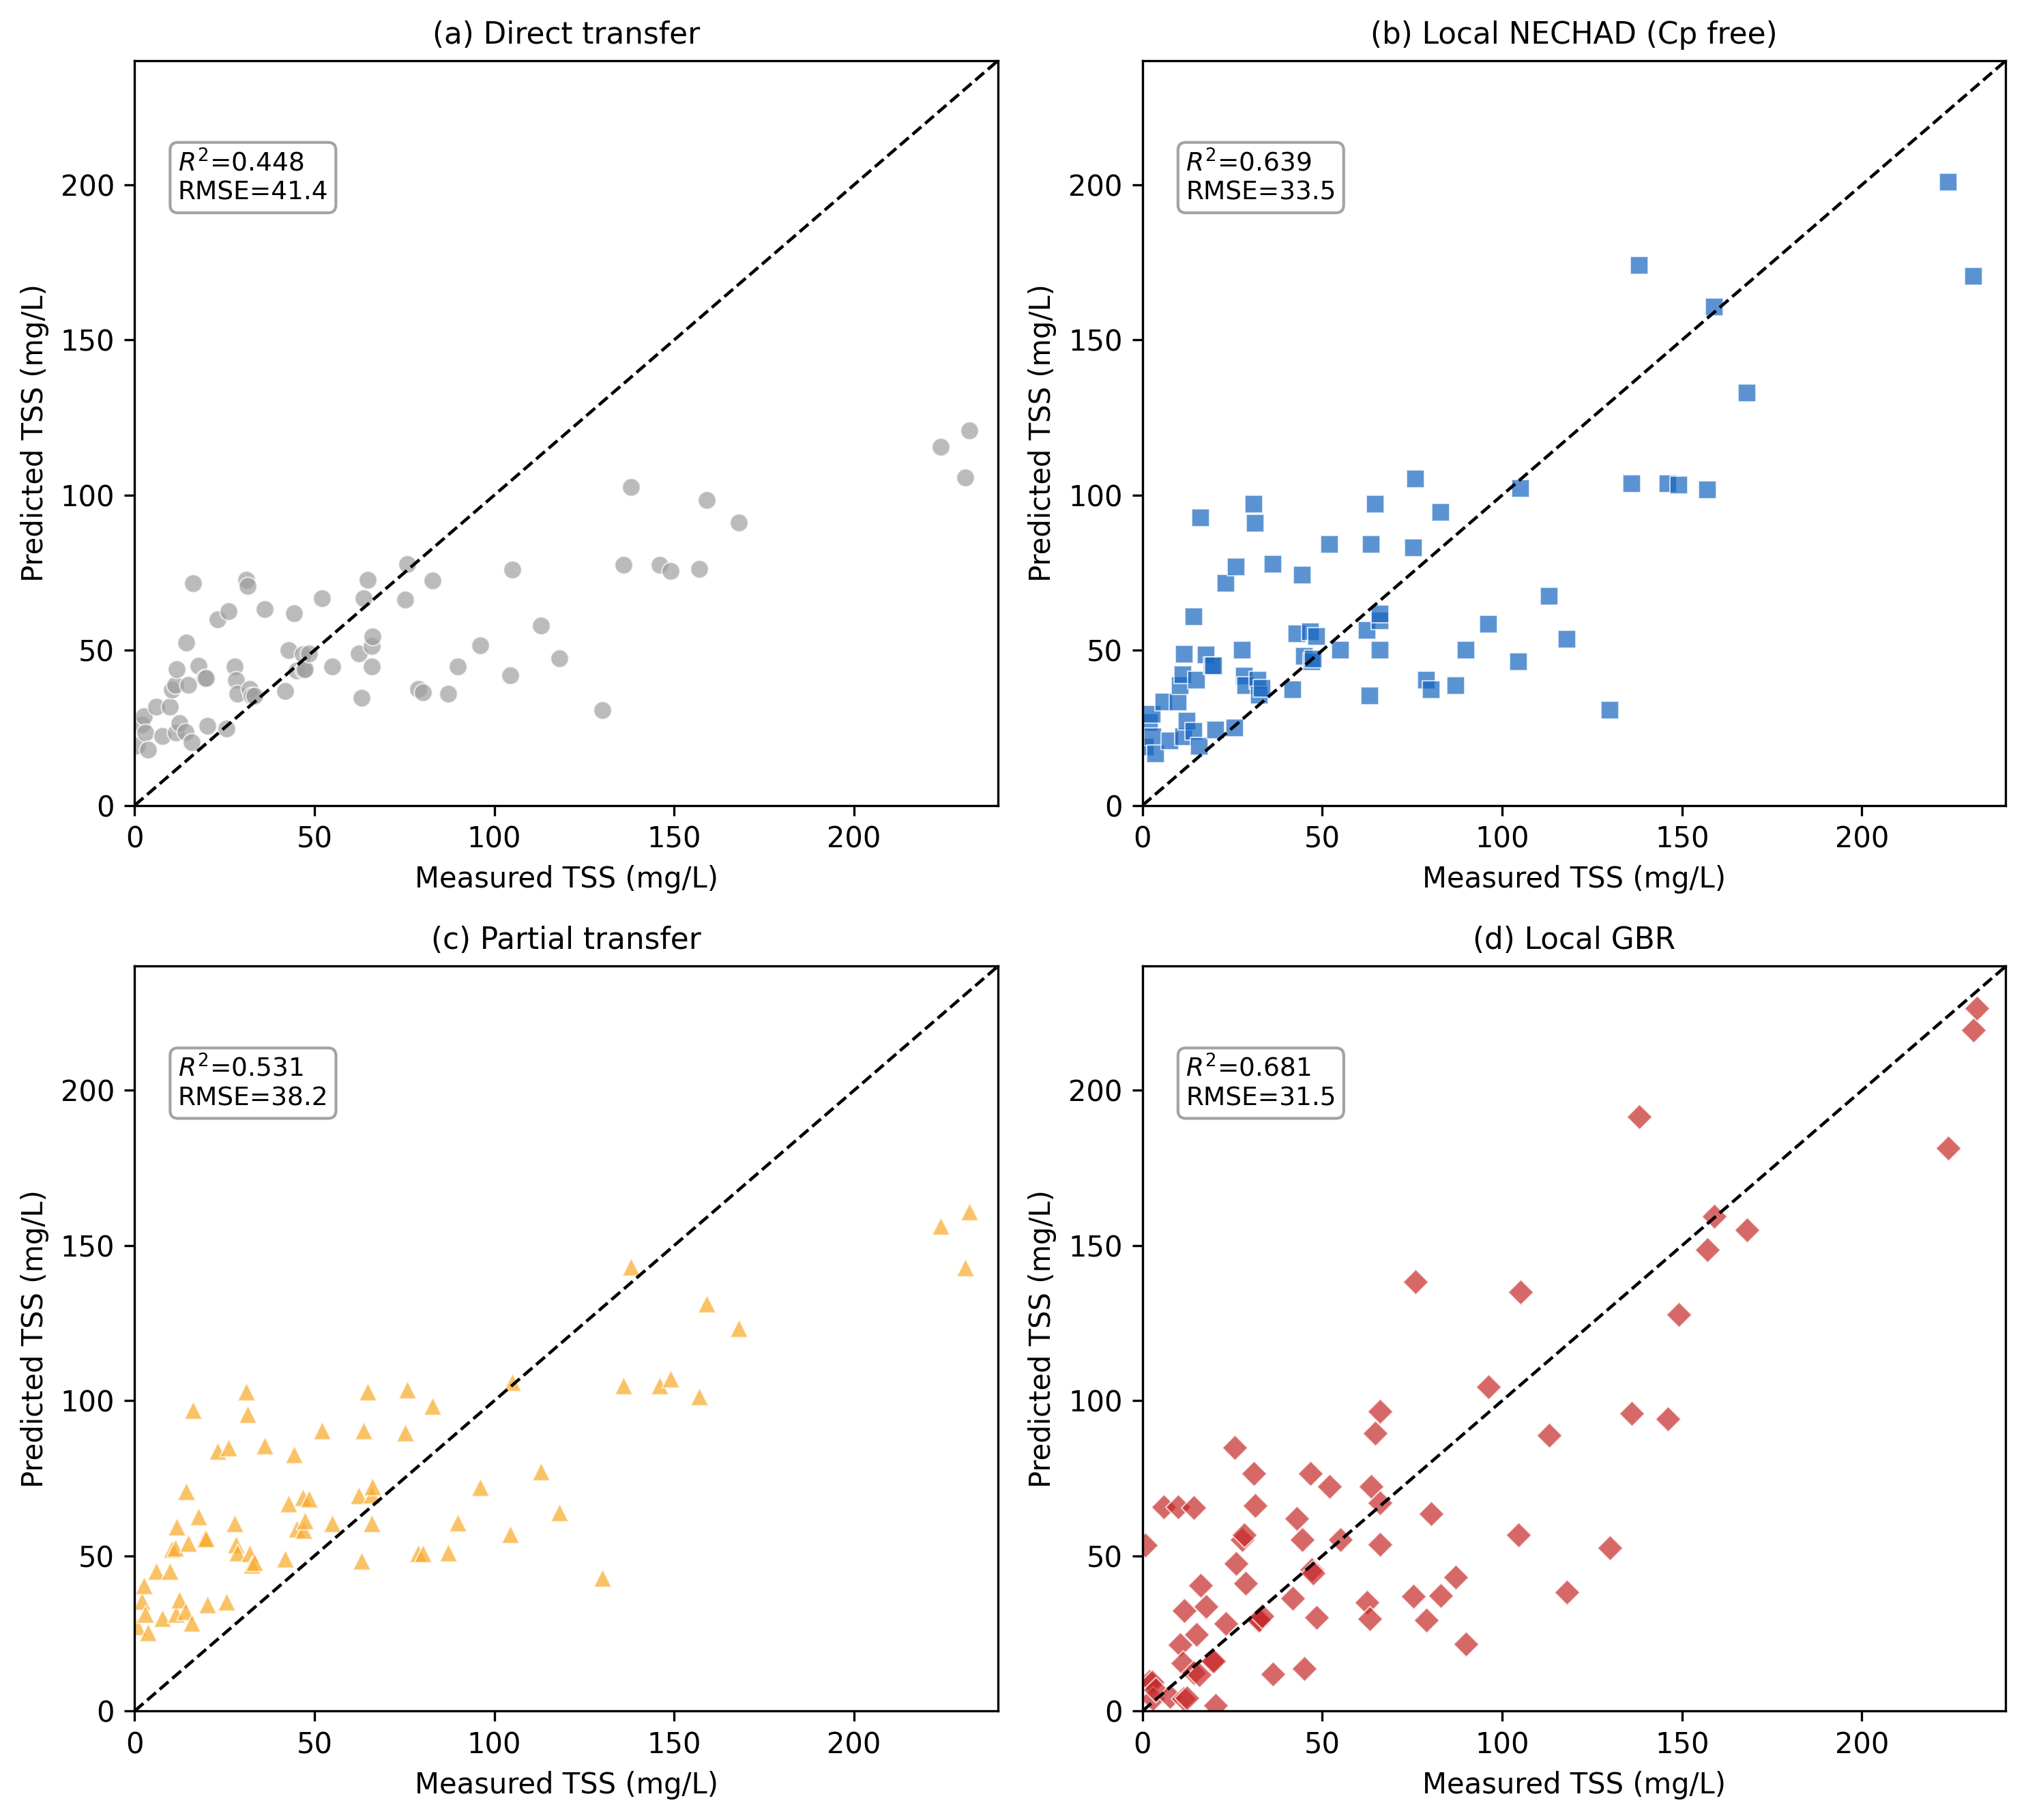
\includegraphics[width=0.95\linewidth]{images/fig3_transferability_scenarios.png}
    \caption{Leave-one-station-out cross-validated observed vs.\
    predicted TSS under four transferability scenarios (CGSM, $n = 74$,
    four monitoring stations). Performance increases with the amount of
    local adaptation permitted (A $<$ C $<$ B $<$ D), with B closely
    approaching the Pajarales Landsat-8 source calibration
    ($R^2 = 0.662$) and no scenario exceeding it.}
    \label{fig:transferability}
\end{figure}
 
 
% ── §3.7 ────────────────────────────────────────────────────────
\subsection{Hydroclimatic Controls on TSS Variability}
\label{sec:results_hydro}
 
Sentinel-1-derived water surface area ranged from 207 to 436~km$^2$
and exhibited a significant increasing trend (Mann--Kendall
$\tau = +0.18$, $p = 0.002$, slope $\approx +1.3$~km$^2$~year$^{-1}$)
over 2015--2025. At the annual scale, S1 water area was significantly
and negatively correlated with annual median TSS at Pajarales
(Pearson $r = -0.766$, $p = 0.010$; Spearman $\rho = -0.733$,
$p = 0.016$; $n = 10$). Higher water extent corresponds to
\emph{lower} TSS --- a freshwater dilution signature. Concurrent with
the increasing S1 water area, surface reflectance declined
significantly (B2: $\tau = -0.31$, $p < 0.001$;
B4: $\tau = -0.27$, $p < 0.001$). These diverging trajectories
suggest a long-term reduction in Magdalena River sediment load.
 
Annual mean ONI was positively associated with annual TSS anomaly
($r = 0.61$, $p = 0.064$, $n = 10$; borderline). The cross-site
coupling between Pajarales and CGSM monthly TSS is strong
($r = 0.777$, $p < 0.001$, $n = 25$ concurrent months).
 
\begin{figure}[h!]
    \centering
    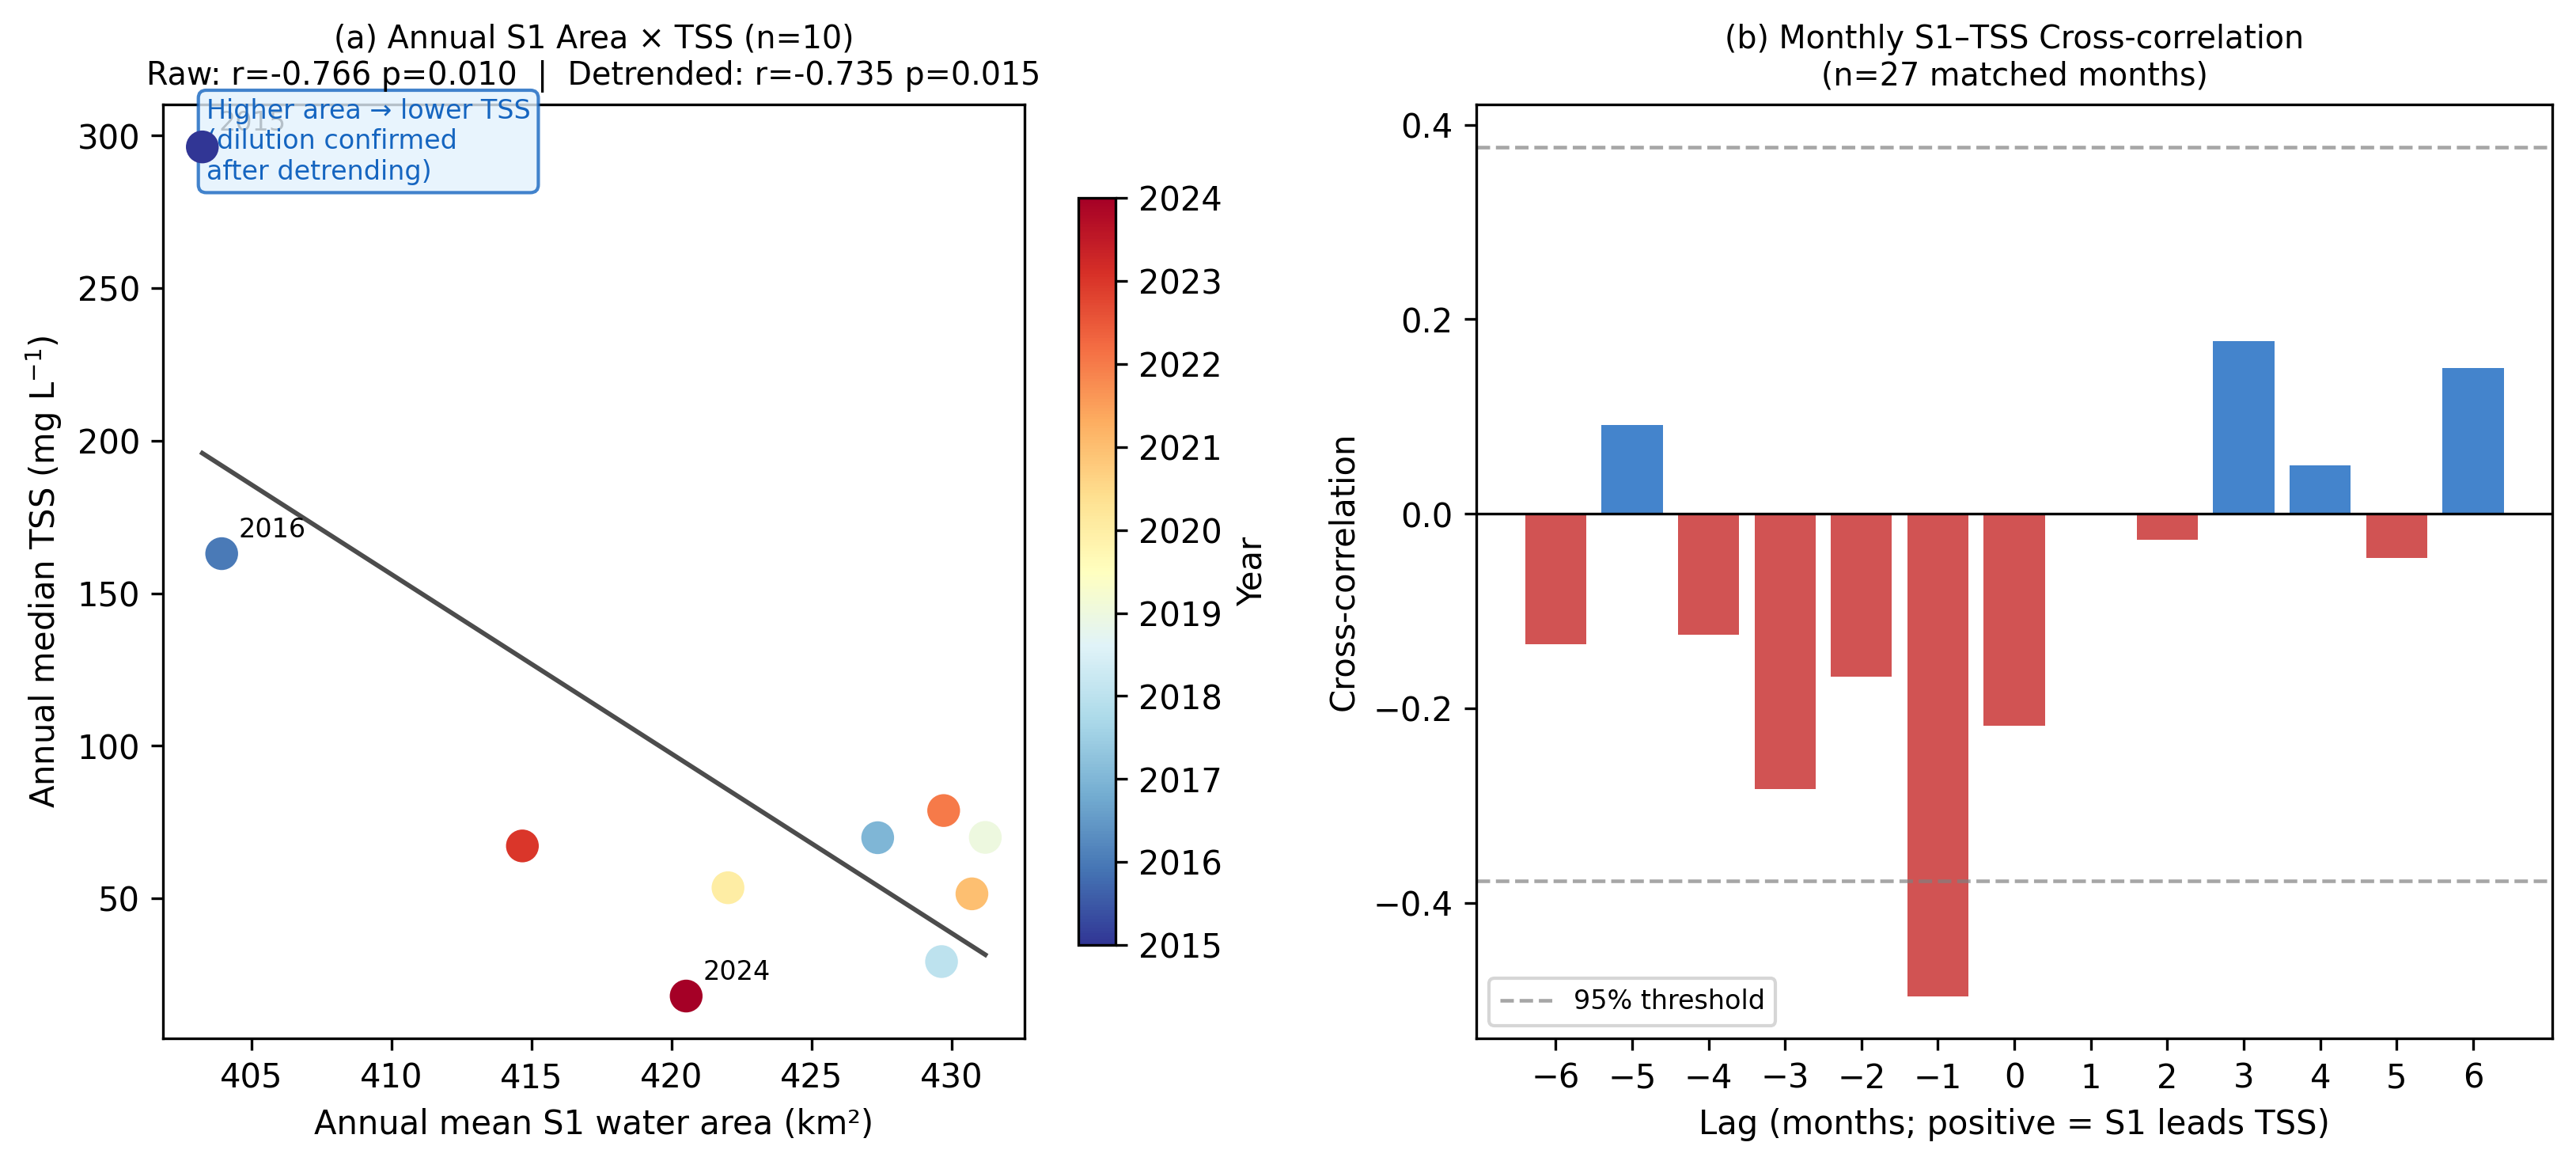
\includegraphics[width=0.95\linewidth]{images/fig7_S1_TSS_verified.png}
    \caption{(a)~Annual S1 water surface area vs.\ annual median TSS
    at Pajarales ($r = -0.766$, $p = 0.010$, $n = 10$). Points
    coloured by ENSO phase. Trend line from linear regression.
    (b)~Normalised cross-correlation between monthly S1 area and
    monthly TSS ($n = 27$ matched months; dashed lines: 95\%
    significance threshold).}
    \label{fig:s1_tss}
\end{figure}
 
\begin{figure}[h!]
    \centering
    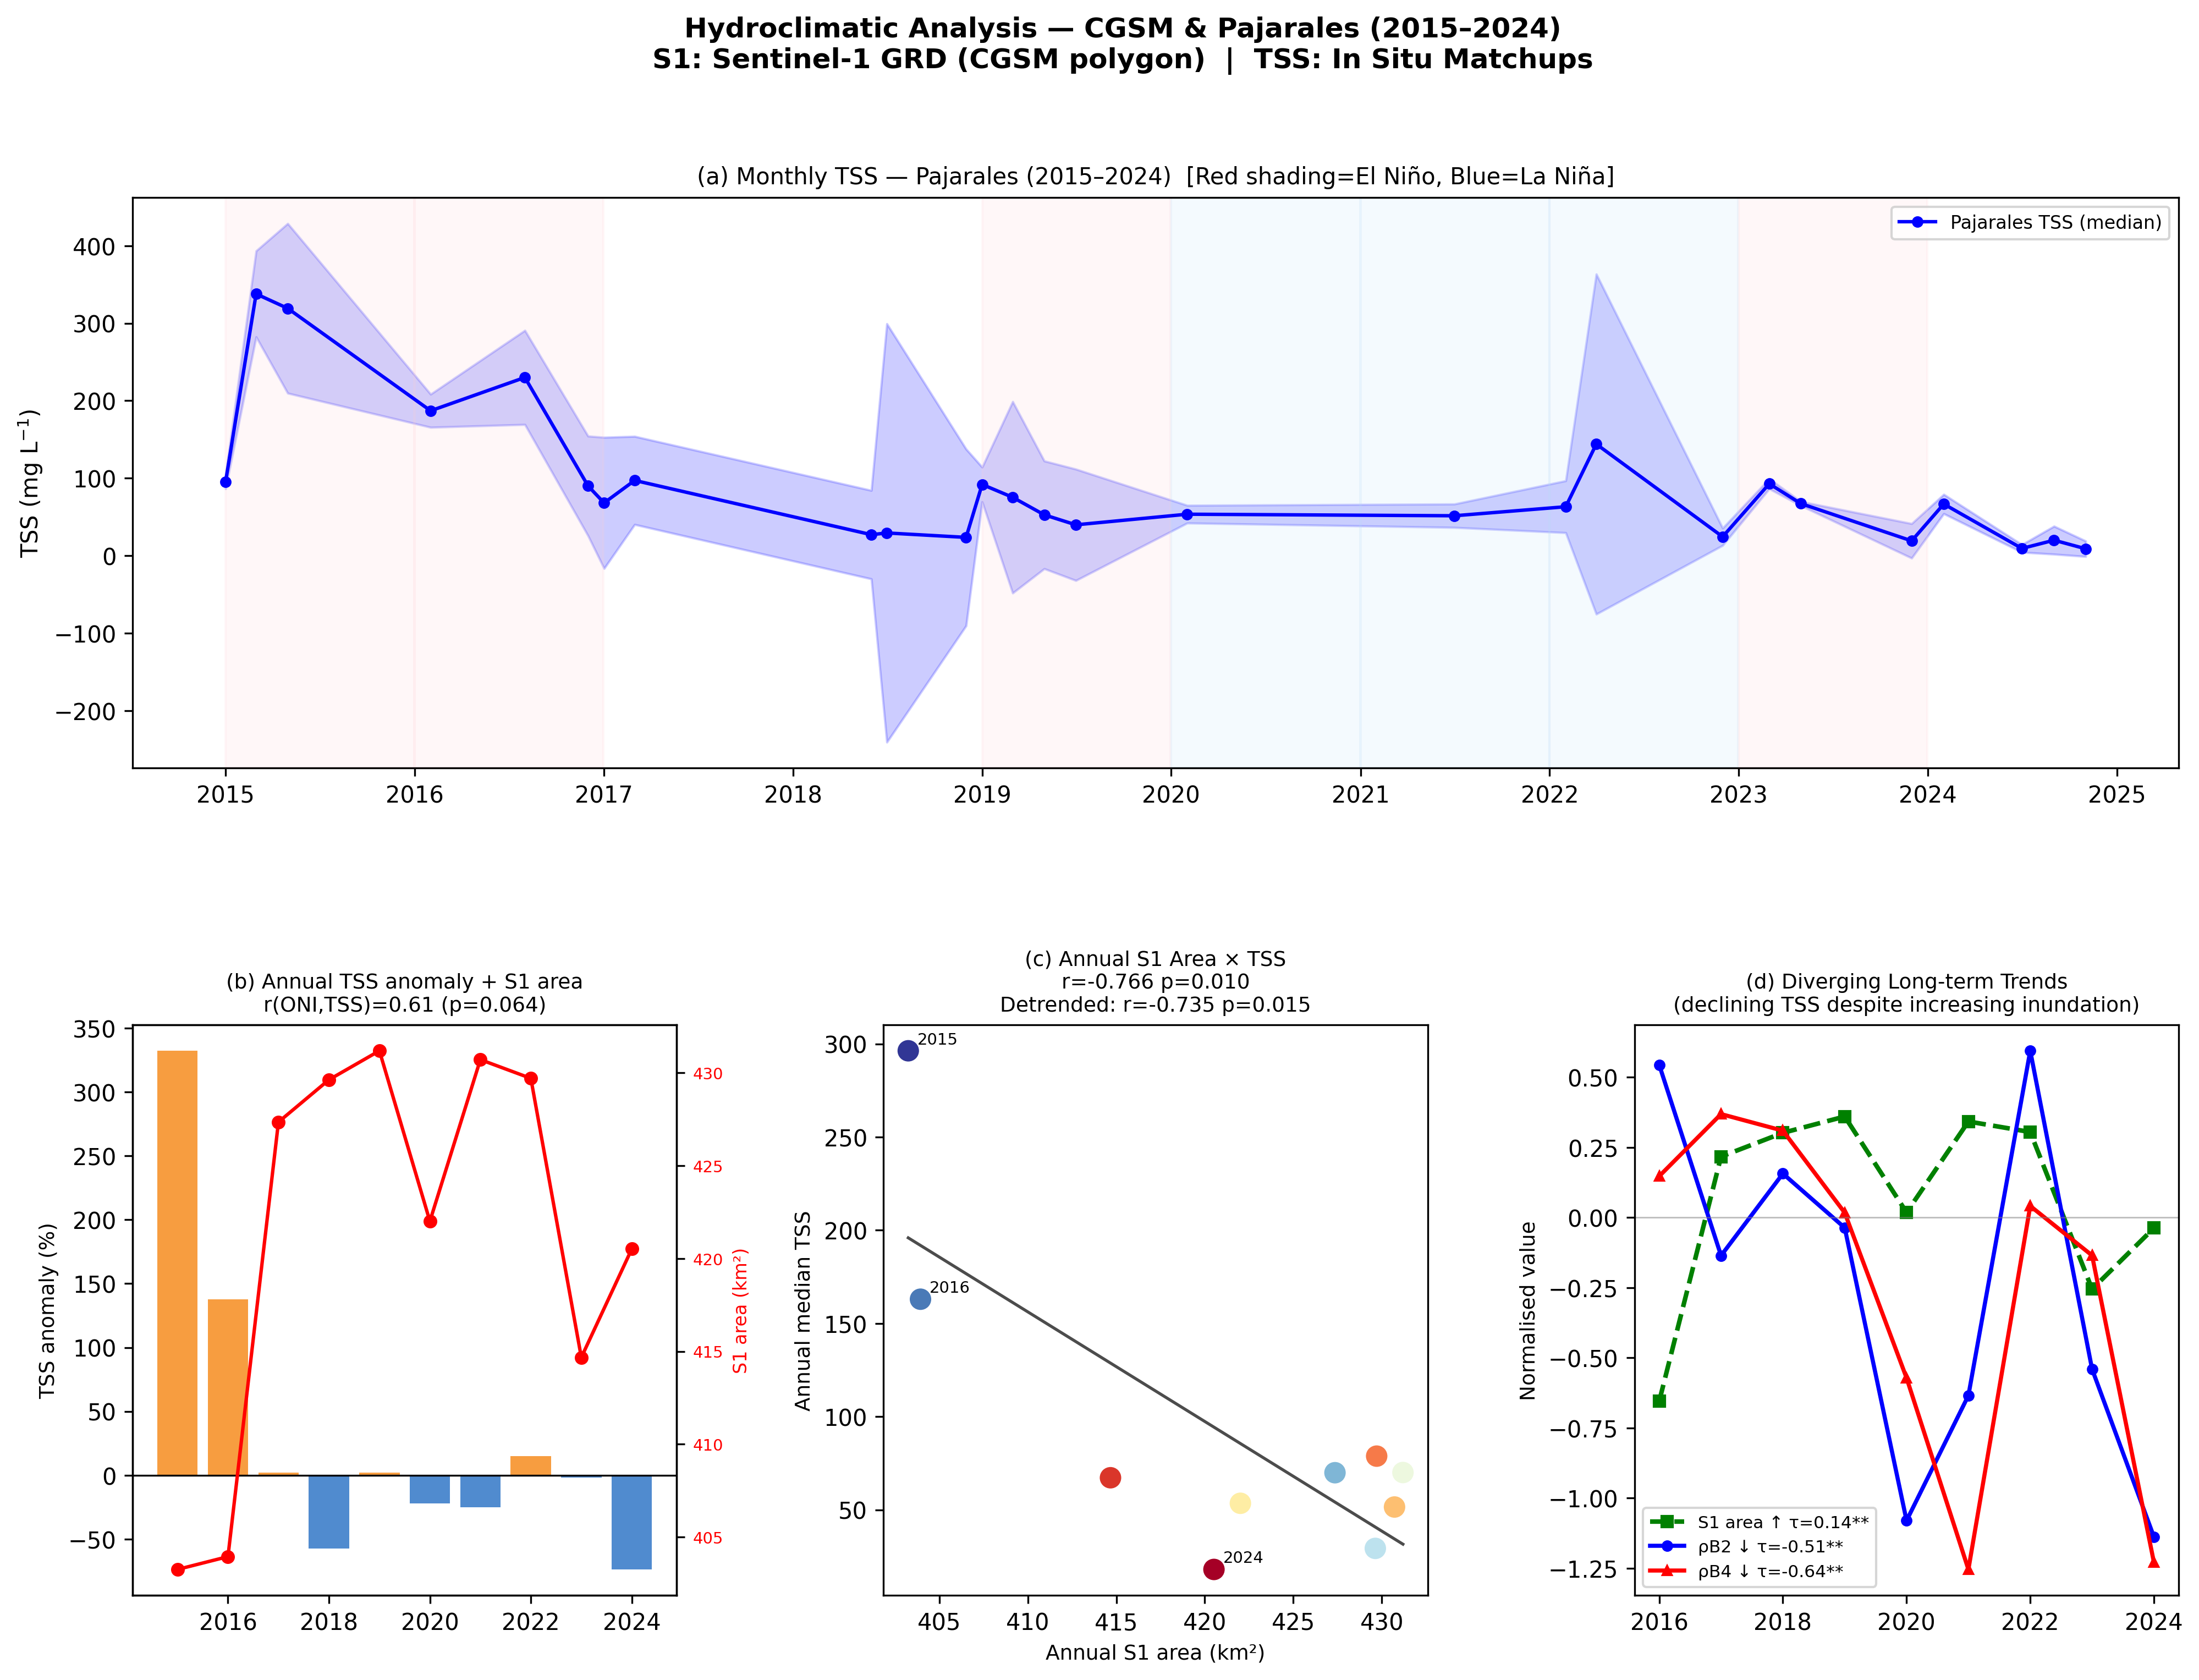
\includegraphics[width=0.95\linewidth]{images/fig8_hydroclimatic_final.png}
    \caption{Hydroclimatic analysis. (a)~Monthly Pajarales TSS and
    ONI index (2015--2026); shading indicates El~Ni\~{n}o (red) and
    La~Ni\~{n}a (blue) phases. (b)~Annual TSS anomaly and mean ONI.
    (c)~Annual S1 water area vs.\ annual TSS ($r = -0.766$,
    $p = 0.010$). (d)~Diverging long-term trends: reflectance
    declining ($\tau < 0$, $p < 0.001$) vs.\ S1 area increasing
    ($\tau = +0.18$, $p = 0.002$). (e)~TSS by ENSO phase
    (Kruskal--Wallis $p = 0.12$).}
    \label{fig:hydroclimatic}
\end{figure}
 
\begin{figure}[h!]
    \centering
    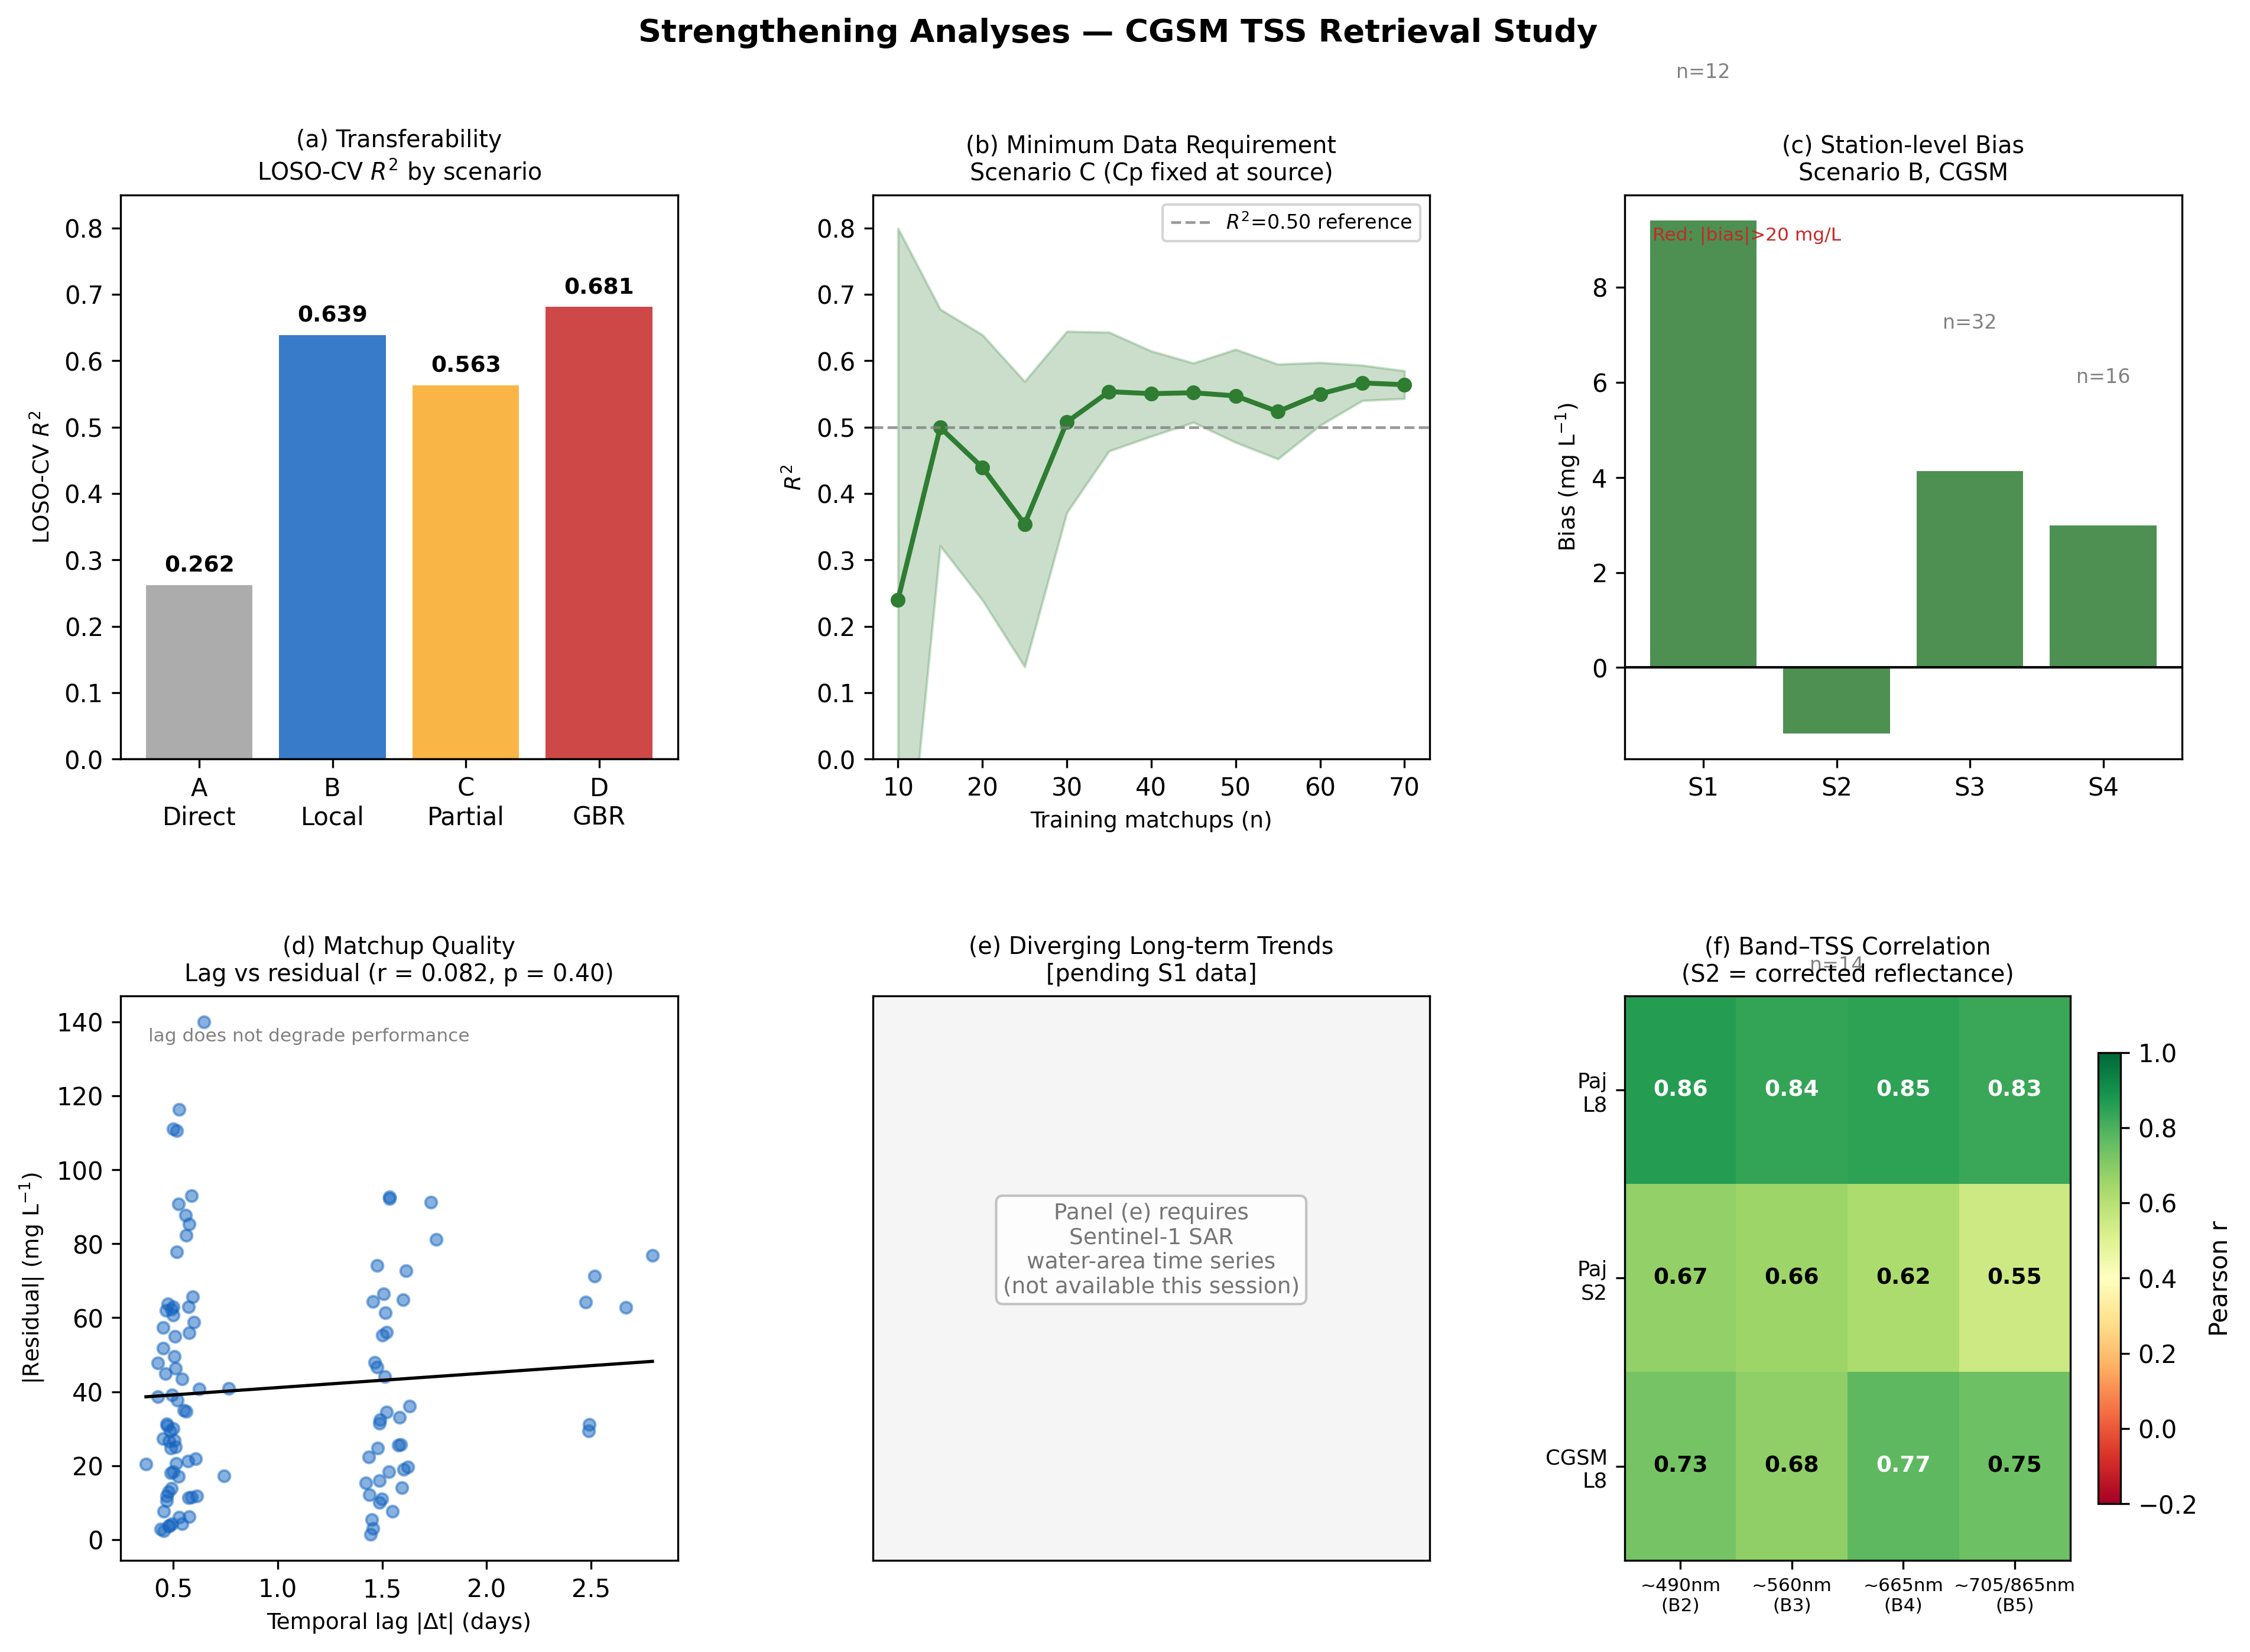
\includegraphics[
        width=0.95\textwidth,
        clip,
        trim=0 0 0 40
    ]{images/fig9_strengthening_analyses.png}
    \caption{Strengthening analyses. (a)~LOSO-CV performance for all
    four transferability scenarios. (b)~Minimum matchup requirement
    for partial transfer (Scenario~C): power curve.
    (c)~Station-level prediction bias at CGSM stations.
    (d)~Temporal lag vs.\ absolute residual ($r = -0.20$,
    $p = 0.08$). (e)~Diverging long-term trends (normalised).
    (f)~Band--TSS Pearson correlation matrix.}
    \label{fig:strengthening}
\end{figure}
 
 
%%%%%%%%%%%%%%%%%%%%%%%%%%%%%%%%%%%%%%%%%%
\section{Discussion}
 
\subsection{Identifiability of Nechad Parameters}
\label{sec:disc_ident}
 
The identifiability analysis reveals that prior $C_p$ values of order
$10^7$ reported for this system reflect optimiser collapse, not valid
calibration. The claim that those values ``remain numerically stable''
is incorrect; an unidentifiable parameter cannot provide reliable
estimates even within the calibration domain.
The correct procedure when $\kappa < 0.35$ is to fix $C_p$ to a value
that is both externally determined and safely outside the system's own
observed reflectance range -- not necessarily the published Nechad
et~al.\ \citeyearpar{NECHAD2010854} value, which can itself sit too
close to, or inside, a given system's reflectance range and destabilise
the fit. In this study, $C_p$ is fixed to the band's physical upper
bound, $C_{p,\text{upper}}$, for this reason, and $A_p$ is estimated
analytically. The same caution extends to the nominal $\kappa \geq 0.35$
case: a free two-parameter fit that converges to the $C_p$ boundary
regardless of initialisation (Sentinel-2 at Pajarales,
Section~\ref{sec:identifiability}) is, in practice, also an
unidentified $C_p$, and is best treated and reported as a
one-parameter fit rather than presented with the appearance of a
genuinely free second parameter. We recommend that future calibration
studies routinely compute and report $\kappa$ alongside model
parameters, verify that any fixed-$C_p$ anchor remains above the
system's observed $\rho_{\max}$, and check optimiser convergence
behaviour across multiple starting values even when $\kappa$ nominally
clears the identifiability threshold.
 
 
\subsection{Model Performance and Uncertainty Sources}
\label{sec:disc_performance}
 
For Landsat-8, in-sample $R^2 = 0.693$ at Pajarales is consistent with,
and slightly exceeds, the leave-one-station-out result
($R^2 = 0.662$), the expected direction of change when moving from
training-set fit to genuine spatial generalisation. The temporal
sensitivity analysis (Section~\ref{sec:sensitivity}) showed that
cross-validated performance is highest at a tighter matchup window
than the one adopted, declining smoothly rather than abruptly as the
window widens to $\pm$2.84~days; the wider window was retained for
sample size and per-station fold stability (Section~\ref{sec:matchup}),
not because it maximises cross-validated $R^2$ in isolation. There is
no significant relationship between temporal lag and absolute residual
within the adopted window ($r = -0.20$, $p = 0.08$), supporting the
temporal weighting strategy (Equation~\ref{eq:weight}) as the
appropriate way to retain, rather than discard, the more temporally
distant matchups that this trade-off admits.
 
\subsubsection{ACOLITE versus Uncorrected Surface Reflectance for Landsat-8}
\label{sec:disc_acolite_vs_raw}
 
An uncorrected Collection-2 Level-2 Landsat-8 reflectance product (raw
digital numbers rescaled by the standard USGS linear transform, with
six aerosol-contaminated acquisitions removed, $n=104$) was evaluated
as an alternative to the ACOLITE-processed product used throughout this
study. The uncorrected product achieved leave-one-station-out
$R^2 = 0.566$--$0.568$ (depending on one- versus two-parameter fitting
mode, which converged to the same result), compared with $R^2 = 0.662$
for the ACOLITE product on the same Pajarales stations. At matched
observations, ACOLITE reflectance showed approximately half the
coefficient of variation of the uncorrected product across every TSS
range examined (0--20, 20--60, 60--150, and 150--700~mg/L), and the
uncorrected product's high-TSS tail ($>$250~mg/L) was non-monotonic
with respect to \textit{in situ} TSS, while ACOLITE's was not. This
indicates that the ACOLITE DSF correction provides genuine noise
suppression for this system rather than performance gains attributable
to dynamic-range compression alone, and supports the use of the
ACOLITE-processed product as the primary Landsat-8 input throughout
this study.
 
 
\subsection{Physical Interpretation of Transferability Results}
\label{sec:disc_transfer}
 
The leave-one-station-out results show a gradient consistent with
genuine, bounded transfer rather than either catastrophic failure or
an implausible inversion: performance improves as more of the model is
allowed to adapt locally, from direct transfer ($R^2 = 0.448$, no
local data used at all) through partial transfer ($R^2 = 0.531$, only
$A_p$ re-estimated locally) to full local recalibration
($R^2 = 0.639$, both parameters free, closely approaching but not
exceeding the Pajarales source calibration's own $R^2 = 0.662$) and the
non-physical GBR ceiling ($R^2 = 0.681$). Critically, no scenario
exceeds the source calibration's cross-validated performance, which
would have been the more concerning pattern, since a transfer target
cannot legitimately outperform the model it was transferred from
without indicating either an evaluation artefact or an unrepresentative
target sample.

Scenario~C does not outperform full local recalibration at this site,
unlike what its physical motivation (a shared, sediment-provenance-
determined $C_p$) might suggest. The explanation is visible in the
reflectance domain itself: CGSM's observed $\rho_{B4}$ range
(0.012--0.071) sits almost entirely below 13\% of $C_{p,\text{upper}}$,
so anchoring $C_p$ there leaves the Nechad curve close to linear over
CGSM's actual operating range and removes the curvature term that
constrains the fit; the locally free $C_p$ in Scenario~B instead
converges to $C_p \approx 0.11$--$0.13$ across leave-one-station-out
folds, much closer to CGSM's own $\rho_{\max}$, giving the fitted curve
usable curvature within the observed domain even though this $C_p$ is
no longer the value Pajarales would suggest. The practical case for
Scenario~C is therefore not an accuracy advantage at this particular
site, but the prospect of better generalisation to a \emph{further}
transfer site with an even narrower reflectance range or fewer local
matchups than CGSM -- a claim this dataset cannot itself test, since
CGSM was the only transfer target available.
 
 
\subsection{Sensor Pooling}
\label{sec:disc_pooling}
 
A pooled single-$A_p$ Nechad fit across both sensors (Landsat-8 and
corrected Sentinel-2 combined, $n=240$) was evaluated against the two
single-sensor fits. The pooled fit achieved in-sample $R^2 = 0.353$,
below both the Landsat-8-only ($R^2 = 0.693$) and Sentinel-2-only
($R^2 = 0.419$) in-sample fits. At matched TSS levels, Sentinel-2
red-band reflectance is approximately 50--85\% higher than Landsat-8
reflectance for the same \textit{in situ} TSS, a persistent offset that
survived the atmospheric-correction fix described in
Section~\ref{sec:disc_s2gap} and that simple band-ratio predictors
(B4/B3, B4/B2, B4 normalised by B2+B3+B4) did not remove; in several
cases these ratios carried opposite-sign correlation with TSS between
the two sensors, ruling them out as sensor-invariant features at this
site. No coincident same-day Landsat-8--Sentinel-2 acquisitions exist
in the matchup dataset to anchor an empirical cross-sensor calibration
directly. Landsat-8 and Sentinel-2 are therefore calibrated and
reported as separate single-sensor models throughout this study
(Table~\ref{tab:pajarales_cv}), with Sentinel-2 recommended primarily
for qualitative spatial/temporal coverage rather than as a
quantitatively equivalent product to Landsat-8.
 
 
\subsection{Sentinel-2 vs.\ Landsat-8 Performance Gap}
\label{sec:disc_s2gap}
 
An initial Sentinel-2 ACOLITE processing run showed a substantially
weaker correlation with \textit{in situ} TSS at Pajarales ($r = 0.118$)
than Landsat-8 ($r = 0.847$). Internal review identified a residual
atmospheric-correction artefact affecting a subset of acquisitions (29
of 130 matchups), consistent with scene-level Rayleigh or sun-glint
over-correction rather than a uniform offset: affected reflectance
values were predominantly compressed or implausibly scaled relative to
neighbouring bands. Following correction, Sentinel-2's correlation with
\textit{in situ} TSS improved to $r = 0.622$ and its leave-one-station-out
$R^2$ improved from $-0.382$ (uncorrected; performance worse than
predicting the sample mean) to $0.372$ (corrected;
Table~\ref{tab:pajarales_cv}).

This correction substantially narrows, but does not close, the
performance gap with Landsat-8 ($R^2_{\text{LOSO}} = 0.662$). The
residual gap does not appear to be explained by simple band-ratio
transformations (B4/B3, B4/(B2+B3+B4), NDTI-type indices): none of
these improved correlation with TSS relative to the raw B4 band for
either sensor, and B4/(B2+B3+B4) in particular carried opposite-sign
correlation with TSS between sensors (Landsat-8: $r = -0.57$;
Sentinel-2: $r = +0.05$), ruling out a simple sensor-invariant
reflectance transform as a near-term fix. We recommend treating S2 and
L8 as separate, single-sensor predictors (Section~\ref{sec:disc_pooling})
and using Sentinel-2 primarily to extend spatial and temporal coverage
between Landsat-8 overpasses in qualitative composites
(Section~\ref{sec:results_spatial}), rather than as a quantitatively
equivalent calibration source, until the remaining gap's physical
origin -- most plausibly continued acquisition-level atmospheric
correction variability -- can be tested directly with near-simultaneous
L8--S2 overpasses and \textit{in-water} radiometric measurements.
 
 
\subsection{Hydroclimatic Drivers of Long-term TSS Variability}
\label{sec:disc_hydro}
 
The analyses in this section are explicitly exploratory: with $n = 27$
matched monthly pairs, the temporal record supports trend detection and
bivariate correlation but not causal attribution or regression
modelling. The findings are reported as preliminary evidence that
motivates a specific, tractable next step (Section~\ref{sec:disc_limits})
rather than as a completed mechanistic analysis.

The significant negative annual S1--TSS correlation ($r = -0.766$,
$p = 0.010$) implies a dilution mechanism: years with greater
inundation correspond to lower TSS owing to sustained freshwater
discharge; years with contracted extent correspond to higher TSS
through concentration effects and wind-driven resuspension
\citep{Blanco2006}. The diverging trends --- S1 area increasing while
reflectance declines --- are inconsistent with a resuspension-dominated
system and point to a reduction in Magdalena River sediment load,
possibly attributable to upstream dam construction, reforestation, or
changing catchment land use. Both patterns are consistent with
hydrological mechanisms reported elsewhere in the CGSM literature
\citep{Blanco2006,Jaramillo2018}; quantifying their relative
contributions requires a continuous, model-derived TSS series from the
full satellite archive, which this study's matchup-limited calibration
cannot yet provide.
 
 
\subsection{Implications for Environmental Monitoring and Management}
\label{sec:disc_management}
 
The satellite-based TSS framework provides a complementary tool to
existing INVEMAR monitoring programmes. The distinct seasonal dynamics
--- dry-season peak at Pajarales ($p < 0.001$) but no significant
seasonal signal at the CGSM ($p = 0.80$) --- have direct management
implications: elevated dry-season turbidity in Pajarales is driven by
wind-driven resuspension and would not be mitigated by hydrological
connectivity restoration in the same way as discharge-driven turbidity.
Scenario~A (direct transfer) already provides a usable zero-local-data
baseline ($R^2 = 0.448$) for rapid deployment to a new CGSM-like
sub-basin; Scenario~C offers a lower-data-requirement option requiring
only local $A_p$ recalibration, at an estimated cost of approximately
20--30 co-located satellite--\textit{in situ} pairs per new sector,
should the modest accuracy gain over direct transfer
(Section~\ref{sec:disc_transfer}) be considered worthwhile relative to
the data collection cost.
 
 
\subsection{Limitations and Future Research Directions}
\label{sec:disc_limits}
 
A fundamental limitation is that all Landsat-8 and CGSM data fall
below $\kappa = 0.35$, making the one-parameter calibration reliant
on the externally-fixed $C_p$ anchor (here, $C_{p,\text{upper}}$) being
appropriate for this system; this was checked directly for Pajarales
(Section~\ref{sec:disc_ident}) but not yet re-verified for CGSM. CGSM
validation remains limited to four stations ($n = 74$), and performance
is therefore reported as point estimates from leave-one-station-out
cross-validation across these four stations rather than as bootstrap
confidence intervals (which would require resampling within already
small per-station folds, and could overstate precision here);
direct station-to-station variability is shown instead in
Figure~\ref{fig:strengthening}c. This four-station validation,
together with the limited number of co-located Sentinel-2 acquisitions
relative to Landsat-8, means the reported scenario gradient
(Section~\ref{sec:results_transfer}) should be treated as indicative of
the right ordering of approaches rather than a precise estimate of
each scenario's accuracy at an arbitrary new site.

The temporal matchup window sensitivity analysis
(Section~\ref{sec:sensitivity}, Figure~\ref{fig:sensitivity}) is
similarly bounded by the assembled matchup pool: it characterises how
performance changes as the window is narrowed from the existing
$\pm$2.84-day ceiling down to $\pm$0.5~days, but cannot independently
test whether a window wider than $\pm$2.84~days would perform better
or worse, since no matchups beyond that lag exist in the dataset. The
$\pm$2.5-day window adopted throughout this study is therefore a
sample-size and fold-stability choice within the available range,
not a verified global optimum.

A second limitation concerns Scenario~C specifically: its proposed
operational advantage rests on a physical argument (shared sediment
provenance constraining $C_p$) that this single-target dataset cannot
accuracy-test, since Scenario~C did not outperform full local
recalibration at CGSM (Section~\ref{sec:disc_transfer}). Confirming or
falsifying its generalisation case requires applying the same four-
scenario framework at additional, sedimentologically similar transfer
targets beyond CGSM.

The Sentinel-2 performance gap was narrowed substantially by correcting
the identified atmospheric-correction artefact
(Section~\ref{sec:disc_s2gap}), but a residual gap relative to
Landsat-8 remains, and its exact physical mechanism still requires
investigation via near-simultaneous L8--S2 overpasses with
\textit{in-water} radiometric measurements. The S1 hydroclimatic
analysis is constrained by bounding box geometry effects; a precise
INVEMAR water-mask shapefile would improve monthly TSS--area
correlations. The matched monthly record ($n = 27$ pairs) supports
bivariate correlations and trend detection but not regression
modelling; extending this to a continuous, satellite-derived TSS time
series (applying the calibrated model to the full 2013--2024 Landsat-8
archive) would provide the sample size needed to partition the
relative contributions of ENSO forcing, river discharge, and
resuspension to interannual TSS variability through a time-series
regression approach.

The transferability framework itself was tested on a single
source-to-target pair: Pajarales and the central CGSM are
hydrologically connected sectors of the same lagoon complex rather
than independent systems. This is a more limited generalization base
than an evaluation across multiple, hydrologically distinct lagoons
would provide, and the framework's applicability to entirely separate
estuarine systems remains to be demonstrated.
 
 
%%%%%%%%%%%%%%%%%%%%%%%%%%%%%%%%%%%%%%%%%%
\section{Conclusions}
 
This study presents a physically grounded, cross-validated framework
for Nechad model calibration and spatial transferability in the
Ci\'enaga Grande de Santa Marta lagoon system. The main conclusions
are:
 
\begin{enumerate}
 
    \item A formal identifiability criterion
    ($\kappa = \rho_{\max}/C_{p,\mathrm{upper}}$) reveals that Landsat-8
    and CGSM data fall below $\kappa = 0.35$, and that Sentinel-2,
    although nominally above this threshold, converges its free $C_p$
    to the same boundary value regardless of optimiser initialisation
    -- making free two-parameter Nechad fitting statistically
    inappropriate for all three site--sensor combinations examined.
    Prior $C_p$ values of order $10^7$ reflect optimiser collapse. The
    closed-form one-parameter estimator is the correct calibration
    procedure for all three, with $C_p$ fixed to the band's physical
    upper bound ($C_{p,\mathrm{upper}}$) rather than the literature
    Nechad et~al.\ \citeyearpar{NECHAD2010854} value, which was found
    to sit inside this system's own observed reflectance range and to
    destabilise the fit (Section~\ref{sec:disc_ident}).
 
    \item Leave-one-station-out cross-validated performance at
    Pajarales is $R^2 = 0.662$ for Landsat-8 and $R^2 = 0.372$ for
    Sentinel-2 (corrected reflectance), evaluated and reported as
    separate single-sensor models; a pooled fit across both sensors
    underperforms either sensor alone (Section~\ref{sec:disc_pooling}).
    Random $k$-fold CV can itself be misleadingly optimistic when
    repeat visits to the same station are split across folds; genuine
    spatial generalisation is better tested by holding out entire
    stations.
 
    \item Direct parameter transfer (Scenario~A) achieves a usable
    zero-local-data leave-one-station-out $R^2 = 0.448$ at the CGSM,
    using the Landsat-8 calibration unchanged. Performance improves
    with the amount of local adaptation permitted: partial transfer
    ($C_p$ fixed, $A_p$ refit locally; $R^2 = 0.531$) and full local
    recalibration (both parameters free; $R^2 = 0.639$), the latter
    closely approaching but not exceeding the Pajarales source
    calibration's own performance ($R^2 = 0.662$); a non-physical
    Gradient Boosting ceiling reaches $R^2 = 0.681$. This ordering
    (A~$<$~C~$<$~B~$\lesssim$~source~$<$~D), with no scenario exceeding
    the source calibration, is the pattern expected of genuine,
    physically bounded transfer.
 
    \item Partial transfer (Scenario~C) does not exceed full local
    recalibration (Scenario~B) at this site, contrary to its physical
    motivation: CGSM's narrow reflectance range sits almost entirely
    below the shared $C_p$ anchor, leaving the curve close to linear
    over the observed domain and removing the curvature information a
    locally free $C_p$ can exploit. Its practical case rests on
    requiring less local data and retaining physical interpretability
    for a \emph{further} transfer site, not on superior accuracy at
    CGSM itself.
 
    \item Pajarales exhibits a statistically significant seasonal TSS
    cycle (dry median 75.3 vs.\ wet 29.3~$mg/L$;
    Kruskal--Wallis $p < 0.001$), while the CGSM shows no significant
    seasonal differentiation ($p = 0.80$), reflecting contrasting
    hydrodynamic regimes between the two sub-lagoon systems.
 
    \item Diverging long-term trends --- S1 water area increasing
    ($\tau = +0.18$, $p = 0.002$) while reflectance declines
    ($\tau = -0.31/-0.27$, $p < 0.001$) --- together with a
    significant negative annual S1--TSS correlation
    ($r = -0.766$, $p = 0.010$), suggest a declining Magdalena River
    sediment load as the dominant driver of long-term water clarity
    improvement in the CGSM.
 
    \item An atmospheric-correction artefact affecting a subset of
    Sentinel-2 acquisitions was identified and corrected, improving
    Sentinel-2's Pajarales correlation with TSS from $r = 0.118$ to
    $r = 0.622$ and its leave-one-station-out $R^2$ from $-0.382$ to
    $0.372$. Even after correction, Sentinel-2 remains substantially
    weaker and less stable than Landsat-8, and a persistent
    inter-sensor reflectance offset (Sentinel-2 reading 50--85\% higher
    than Landsat-8 at matched TSS) is not removed by simple band-ratio
    transforms, precluding pooled multi-sensor calibration at this
    site; Landsat-8 is recommended as the primary quantitative product
    and Sentinel-2 as a qualitative coverage supplement.

\end{enumerate}
 
These results provide a reproducible calibration and transfer framework
applicable to other data-limited tropical coastal lagoons where a
sedimentologically similar calibration site exists and the
identifiability conditions described here can be verified, though this
study demonstrates the approach on a single, hydrologically connected
source-to-target pair; validation across independent lagoon systems is
needed before broader generalization can be claimed.

%%%%%%%%%%%%%%%%%%%%%%%%%%%%%%%%%%%%%%%%%%
\vspace{6pt} 

\authorcontributions{Conceptualization, J.R., L.J.O.\ and A.B.; Methodology, J.R.; Software, J.R.; Validation, J.R., L.J.O., A.C.T.-E.\ and J.C.R.; Formal Analysis, J.R.; Investigation, J.R.\ and A.C.T.-E.; Resources, L.J.O.\ and J.C.R.; Data Curation, J.R.; Writing -- Original Draft Preparation, J.R.; Writing -- Review \& Editing, L.J.O., A.C.T.-E., J.C.R.\ and A.B.; Visualization, J.R.; Supervision, L.J.O.\ and A.B.; Project Administration, A.B.; Funding Acquisition, L.J.O.\ and A.B. All authors have read and agreed to the published version of the manuscript.}

\funding{[PLACEHOLDER -- no funding statement was present in the source draft. Insert the appropriate statement here, e.g. ``This research received no external funding.'' or ``This research was funded by [funder name], grant number [xxx].'' Funding details should also be entered separately in the submission system.]}

\institutionalreview{Not applicable. This study did not involve human participants, human data, human tissue, or animals; all data were derived from remote sensing imagery and previously collected institutional water-quality monitoring records.}

\informedconsent{Not applicable.}

\dataavailability{Satellite imagery used in this study is publicly available from the United States Geological Survey (USGS) EarthExplorer (Landsat 8) and the Copernicus Open Access Hub (Sentinel-1 and Sentinel-2). 
The Oceanic Niño Index (ONI) data were obtained from the National Oceanic and Atmospheric Administration (NOAA).
In situ TSS measurements were provided by INVEMAR and are subject to institutional data-sharing policies.
Derived products, including satellite-based TSS estimates, water extent time series, and merged analysis datasets, are available from the corresponding author upon reasonable request.
The full code used for atmospheric correction, mosaicking, calibration, and time--series analysis is available in a public repository: GitHub repository, \url{https://github.com/USER/CGSM-TSS-Analysis}; DOI archived version (Zenodo), \url{https://doi.org/10.5281/zenodo.XXXXXXX}. [PLACEHOLDER -- replace with the final repository URL and DOI before submission.]}
 
\acknowledgments{The authors acknowledge INVEMAR for providing in situ water quality data used in this study.
We also acknowledge the United States Geological Survey (USGS), the European Space Agency (ESA), and the National Oceanic and Atmospheric Administration (NOAA) for open access to satellite and climate datasets.}


\conflictsofinterest{The authors declare no conflicts of interest. The funders had no role in the design of the study; in the collection, analyses, or interpretation of data; in the writing of the manuscript; or in the decision to publish the results.}


%%%%%%%%%%%%%%%%%%%%%%%%%%%%%%%%%%%%%%%%%%
\abbreviations{Abbreviations}{
The following abbreviations are used in this manuscript:
\\

\noindent 
\begin{tabular}{@{}ll}

CGSM & Cienaga Grande de Santa Marta\\
TSS & Total Suspended Solids\\
ENSO & El Niño-Oscilación del Sur\\
ONI & Oceanic Niño Index\\
SAR & Synthetic Aperture Radar\\
S2 & Sentinel 2 (A-B) sensors\\
L8 & Landsat 8 sensor
\end{tabular}
}

%%%%%%%%%%%%%%%%%%%%%%%%%%%%%%%%%%%%%%%%%%
\begin{adjustwidth}{-\extralength}{0cm}

\reftitle{References}

\bibliography{ref}       % sin la extensión .bib


%%%%%%%%%%%%%%%%%%%%%%%%%%%%%%%%%%%%%%%%%%
\PublishersNote{}
\end{adjustwidth}
\end{document}
